\PassOptionsToPackage{hidelinks}{hyperref}

\documentclass[book,twoside,openright]{StylesAndSettings/thesis}
\setlength{\footskip}{9mm}
%\usepackage[round]{cite}				 %Allows abbreviated numerical citations.
\usepackage{pdfpages}			 %Allows you to include full-page pdfs.
\usepackage{wrapfig}			 %Lets you wrap text around figures.
\usepackage{bm} 				 %Bolded maths characters.
\usepackage{upgreek}			 %Upright Greek characters.
\usepackage{dsfont}				 %Double-struck fonts.
\usepackage{simplewick}			 %For typesetting Wick contractions.
\usepackage{mathtools}		     %Can be used to fine-tune the maths presentation.	
\usepackage{framed}			     %For boxed text.
\usepackage{microtype}			 %pdfLaTeX will fix your kerning.
\usepackage{marvosym}			 %Include symbols (like the Euro symbol, etc.).
\usepackage{color}				 %Nice for scalable pdf graphics using Inkscape.
\usepackage{transparent}	     %Nice for scalable pdf graphics using Inkscape.
\usepackage{placeins}			 %Lets you put in a \FloatBarrier to stop figures floating past this command.
\usepackage{mdframed,mdwlist}    %Use these for nice lists (less white space).
\usepackage{float}               %Improved interface for floating objects. 
\usepackage{mathdots}            %Changed the basic LaTeX and plain TeX commands.
\usepackage{eucal}               %Font shape definitions to use the Euler script symbols in math mode.
\usepackage{listings}
\usepackage{array}               %Extending the array and tabular environments.
\usepackage{stmaryrd}            %The StMary’s Road symbol font.
\usepackage{pifont}              %Access to PostScript standard Symbol and Dingbats fonts.
\usepackage{lipsum}    
%Easy access to the Lorem Ipsum sample text.
\usepackage{etoolbox}
\usepackage{enumerate}           %Enumerate with redefinable labels.
\usepackage[all]{xy}             %This is a special package for drawing diagrams.
\usepackage[utf8]{inputenc}      %Makes all displayable utf8 characters available as input.
\usepackage{csquotes}
\usepackage{shellesc}
\usepackage{fancyhdr}            %Extensive control of page headers and footers.
\usepackage{blindtext}           %Produced 'blind' text for testing.
\usepackage{tikz}                %To create graphic elements.
\usepackage{amsmath}
\usetikzlibrary{shapes.geometric, arrows}
\usepackage[figuresright]{rotating}	%Allows large tables to be rotated to landscape.
\usepackage{chngcntr} % Allows tables to not include chapter numbers
%You can add more packages here if you need
\usepackage{caption} % Allows caption formatting to be customised
\usepackage{titlesec} % Added for changing heading and title spacing
\usepackage[style=apa, backend=biber, natbib=true]{biblatex}
\DeclareLanguageMapping{american}{american-apa}
\addbibresource{./References/References.bib}
\bibliography{References/References}

%This defines some macros that implement Latin abbreviations
%COMMENT OUT OR DELETE IF UNDESIRED.
\newcommand{\via}{\textit{via}} %Italicised via.
\newcommand{\ie}{\textit{i.e.}} %Literally.
\newcommand{\eg}{\textit{e.g.}} %For example.
\newcommand{\etc}{\textit{etc.}} %So on...
\newcommand{\vv}{\textit{vice versa}} %And the other way around.
\newcommand{\viz}{\textit{viz}.} %Resulting in.
\newcommand{\cf}{\textit{cf}.} %See, or 'consistent with'.
\newcommand{\apr}{\textit{a priori}} %Before the fact.
\newcommand{\apo}{\textit{a posteriori}} %After the fact.
\newcommand{\vivo}{\textit{in vivo}} %In the flesh.
\newcommand{\situ}{\textit{in situ}} %On location.
\newcommand{\silico}{\textit{in silico}} %Simulation.
\newcommand{\vitro}{\textit{in vitro}} %In glass.
\newcommand{\vs}{\textit{versus}} %James \vs{} Pete.
\newcommand{\ala}{\textit{\`{a} la}} %In the manner of...
\newcommand{\apriori}{\textit{a priori}} %Before hand.
\newcommand{\etal}{\textit{et al.}} %And others, with correct punctuation.
\newcommand{\naive}{na\"\i{}ve} %Queen Amidala is young and \naive{}.

\usepackage[T1]{fontenc}
\usepackage[english,polish]{babel}

\PassOptionsToPackage{headheight=14pt,binding offset=5mm}{geometry}
\usepackage{fancyhdr}

\fancyhf{}
\fancyhead[LO]{\nouppercase{\rightmark}}
\fancyhead[RE]{\nouppercase{\leftmark}}
\fancyhead[LE,RO]{\thepage}
\pagestyle{fancy}

\addto\captionspolish{\renewcommand{\appendixname}{Appendix}} 

% Requires: \usepackage{hyperref} (load it near the end of your preamble)
\makeatletter
\newcommand{\AppChapter}[1]{%
  \refstepcounter{chapter}% A, B, C...
  \setcounter{section}{0}%
  % Printed heading: "Appendix A: Title"
  \chapter*{\appendixname~\thechapter \ #1}%
  % Define the clickable anchor exactly here:
  \Hy@raisedlink{\hyper@anchorstart{chapter.\theHchapter}\hyper@anchorend}%
  % PDF bookmark (outline)
  \pdfbookmark[0]{\appendixname~\thechapter}{chapter.\theHchapter}%
  % TOC entry: ONLY "Appendix A", linked to that anchor
  \addtocontents{toc}{%
    \protect\contentsline{chapter}{\appendixname~\thechapter}{\thepage}{chapter.\theHchapter}}%
  % Running heads (optional)
  \markboth{\appendixname~\thechapter}{\appendixname~\thechapter}%
}
\makeatother

\usepackage{url}

\setcounter{biburllcpenalty}{7000}
\setcounter{biburlucpenalty}{8000}


\title{PiS as Mnemonic Warriors \\
\Large A Comporative Analysis of Changes and Continuity of Memory Narratives in the Election Campaigns 2015 and 2023}
\author{Viktoria Rybicki, BA}
\date{\{year\}}

\let\oldaddcontentsline\addcontentsline
\renewcommand{\addcontentsline}[3]{}

\begin{document}

% -- helper: force & just within a group --
\newcommand{\blxampdelims}{%
  \DeclareDelimFormat{finalnamedelim}{\addspace\&\space}%
  \DeclareDelimFormat{multinamedelim}{\addspace\&\space}%
}

% Parenthetical: (Author1 & Author2, 1989)
% - break allowed BEFORE the citation if needed
% - citation itself is unbreakable
\DeclareCiteCommand{\citeplink}
  {\usebibmacro{prenote}}
  {%
    \penalty0 % allow a break right before the citation if it won't fit
    \mbox{%
      \mkbibparens{%
        \begingroup
          \blxampdelims
          \bibhyperref{\printnames{labelname}}%
        \endgroup
        \addcomma\space
        \bibhyperref{\printfield{labelyear}\printfield{extrayear}}%
      }%
    }%
  }
  {\multicitedelim}
  {\usebibmacro{postnote}}

% Textual: Author1 & Author2 (1989)
\DeclareCiteCommand{\citetlink}
  {\usebibmacro{prenote}}
  {%
    \penalty0
    \mbox{%
      \begingroup
        \blxampdelims
        \bibhyperref{\printnames{labelname}}%
      \endgroup
      \space
      \mkbibparens{\bibhyperref{\printfield{labelyear}\printfield{extrayear}}}%
    }%
  }
  {\multicitedelim}
  {\usebibmacro{postnote}}

% Possessive: Author’s (1989)
\DeclareCiteCommand{\posscite}
  {\usebibmacro{prenote}}
  {%
    \penalty0
    \mbox{%
      \begingroup
        \blxampdelims
        \bibhyperref{\printnames{labelname}}%
      \endgroup
      's\space
      \mkbibparens{\bibhyperref{\printfield{labelyear}\printfield{extrayear}}}%
    }%
  }
  {\multicitedelim}
  {\usebibmacro{postnote}}

% --- \citemultp{keyA,keyB,...} ---
\makeatletter
\newcommand{\citemultp}[1]{%
  \mkbibparens{%
    \begingroup
      \def\citemultp@sep{}%
      \forcsvlist{\citemultp@print}{#1}%
    \endgroup
  }%
}
\newcommand{\citemultp@print}[1]{%
  \citemultp@sep
  \entrydata*{#1}{%
    \penalty0 % allow a break before this item
    \mbox{%
      \bibhyperref{%
        \begingroup
          \blxampdelims
          \printnames{labelname}%
        \endgroup
        \addcomma\space
        \printfield{labelyear}\printfield{extrayear}%
      }%
    }%
  }%
  \def\citemultp@sep{; \space}%
}
\makeatother

% Make natbib-style command names use these:
\let\parencite\citeplink   % so \citep{...} works
\let\textcite\citetlink    % so \citet{...} works


\renewcommand{\hbar}{\mathchar'26\mkern-7.5mu h}

\frontmatter
\maketitle
\clearpage
\setcounter{page}{1}
\pagenumbering{roman}

\pagestyle{plain}
\section
\normalfont
{\bfseries{Field of Studies}} \\
European Studies \\

\noindent
{\bfseries{In Partial Fulfilment of the Requirements for the Degree of}} \\
\noindent
{\textit{Magister (mgr)}} of European Studies (Central and East European, Russian and Eurasian Studies):
Jagiellonian University, Poland \\

\noindent
{\textit{International Master’s (IntM)}} in Central and East European, Russian and Eurasian Studies:
University of Glasgow, UK  \\

\noindent
{\textit{Master of Arts in Social Sciences (MA)}} in Central and East European, Russian and Eurasian Studies: University of Tartu, Estonia \\

\noindent
{\bfseries{Word count of this thesis}} \\
\noindent
$\approx$ 23450 words excluding abstract, footnotes and bibliography \\

\vspace{2cm}

\noindent
{\bfseries{Authorship Declaration}} \\
\noindent
I have prepared this thesis independently. All the views of other authors, as well as data from literary sources and elsewhere, have been cited. \\

\vspace{1cm}

\noindent
Viktoria Rybicki, 25/08/2025 \\

\clearpage

\dedication{To my fianceé, my friends and family \\ Thank you for your love and support}
\clearpage

\newpage\null\thispagestyle{empty}\newpage

\pagestyle{fancyplain}
\normalfont
\section*{Abstract}

In contemporary Poland, the politics of memory have emerged as a key site of national identity formation and political legitimacy. The Law and Justice Party (PiS) has emerged as a pivotal political force in shaping historical narratives, rendering collective memory a tool of governance, a means of exclusion, and a device for populist mobilisation. While attempts to post-communist European memory politics have continued to rise, comparative, digital, and discourse analyses of how mnemonic narratives evolve within the same political party over time remain rare. This thesis examines how PiS has served as a "mnemonic warrior" during the 2015 and 2023 election campaigns by analysing how narratives of victimhood, betrayal, and national purity are constructed, reinterpreted, and disseminated through both traditional and new media. Using a mixed-methods design combining Critical Discourse Analysis (CDA) and Digital Ethnography, the study examines party manifestos, media coverage, and social media accounts. The research employs the Discourse-Historical Approach to CDA and uses tools such as 4CAT and Zeeschuimer for gathering and analysing online material. Through examination, clear consistency in PiS's practices of memory is identifiable, and these hinge upon selective victimhood, elite delegitimisation, and historical revisionism. But the 2023 campaign demonstrates an intensification of digital approaches, particularly on X (formerly Twitter), where previous stories are re-authored in emotive, moralising, and exclusionary narratives aimed at constructing a closed memory community. The study contributes to the understanding of right-wing populist actors weaponising memory to advance polarisation and suppress pluralism. It highlights the necessity of temporally comparative and interdisciplinary study of memory politics, particularly in relation to increasing influence.

\vfill

\noindent\textbf{Keywords:} Collective Memory, Critical Discourse Analysis (CDA), Digital Ethnography, Law and Justice Party (PiS), Memory Politics, Mnemonic Warrior, Othering, Populism, Victimhood

\newpage\null\thispagestyle{empty}\newpage

\section*{Streszczenie}
We współczesnej Polsce polityka pamięci stała się kluczowym elementem kształtowania tożsamości narodowej i legitymizacji politycznej. Partia Prawo i Sprawiedliwość (PiS) stała się kluczową siłą polityczną w kształtowaniu narracji historycznych, czyniąc pamięć zbiorową narzędziem rządzenia, środkiem wykluczenia i instrumentem mobilizacji populistycznej. Podczas gdy próby postkomunistycznej europejskiej polityki pamięci nadal nasilają się, analizy porównawcze, cyfrowe i dyskursywne dotyczące ewolucji narracji mnemonicznych w ramach tej samej partii politycznej w miarę upływu czasu pozostają rzadkością. W niniejszej pracy przeanalizowano, w jaki sposób PiS pełniło rolę „wojownika pamięci” podczas kampanii wyborczych w 2015 i 2023 r., analizując sposób konstruowania, reinterpretacji i rozpowszechniania narracji o ofiarach, zdradzie i czystości narodowej zarówno w mediach tradycyjnych, jak i nowych. Wykorzystując metodę mieszaną, łączącą krytyczną analizę dyskursu (CDA) i etnografię cyfrową, badanie analizuje manifesty partyjne, relacje mediów i konta w mediach społecznościowych. W badaniach zastosowano podejście dyskursowo-historyczne do CDA oraz narzędzia takie jak 4CAT i Zeeschuimer do gromadzenia i analizowania materiałów internetowych. W wyniku analizy można dostrzec wyraźną spójność w praktykach PiS dotyczących pamięci, które opierają się na selektywnym traktowaniu ofiar, delegitymizacji elit i rewizjonizmie historycznym. Jednak kampania z 2023 r. wykazuje intensyfikację działań w mediach cyfrowych, zwłaszcza na platformie X (dawniej Twitter), gdzie wcześniejsze historie są przerabiane na emocjonalne, moralizatorskie i wykluczające narracje mające na celu stworzenie zamkniętej społeczności pamięci. Badanie przyczynia się do zrozumienia, w jaki sposób prawicowi populiści wykorzystują pamięć do pogłębiania polaryzacji i tłumienia pluralizmu. Podkreśla ono konieczność prowadzenia porównawczych i interdyscyplinarnych badań nad polityką pamięci, szczególnie w kontekście jej rosnącego wpływu.

\vfill

\noindent\textbf{Słowa kluczowe:} Etnografia cyfrowa, Inność, Krytyczna analiza dyskursu (CDA), Ofiarowość, Pamięć zbiorowa, Polityka pamięci, Populizm, Prawo i Sprawiedliwość (PiS), Wojownik Mnemonic

\newpage\null\thispagestyle{empty}\newpage

\clearpage
\let\cleardoublepage=\clearpage 

\selectlanguage{english}
\tableofcontents

\let\addcontentsline\oldaddcontentsline

\pagenumbering{arabic}

\mainmatter

\newpage\null\thispagestyle{empty}\newpage
\newpage\null\thispagestyle{empty}\newpage

\setlength{\parindent}{0in}
\setlength{\parskip}{\baselineskip}

\raggedbottom

%CHAPTER 1
\chapter[Introduction]{Introduction}
\label{Chap:Introduction}

Since 2005, Poland's Law and Justice Party (PiS) has actively worked to reshape the country's memory. PiS has used laws, institutions, and symbolic actions to turn memory into a tool of political power. This approach simplifies history by dividing people into heroes and traitors, serving a specific ideological agenda \citep{lazor_memory_2016}. Under PiS, memory becomes a space where the state’s version of history is enforced, alternative views are silenced, and national identity is reshaped around a narrative of victimhood \citep{stanczyk_commemorating_2014}.

These dynamics can be explained by the theory of "mnemonic narratives", which are selective and structured representations of the past that are shaped and shared within political, institutional, and cultural contexts \citep{assmann_transnational_2014}. Memory is not fixed; it is constantly reshaped in political contexts and serves both as a performance and as a means of setting norms \citep{olick_social_1998}. Mnemonic narratives are not just about recalling the past; they are tools of power that shape group identity and justify authority \citep{bernhard_notitle_2014}.

Within this context, the Law and Justice party (PiS) operates as a "mnemonic warrior", a political actor that strategically uses memory to assert dominance over national narratives. Rather than engaging in an honest reflection on the past, PiS treats memory politics as a battleground where competing actors fight to impose singular, unchallenged interpretations of history. This more exclusionary and combative approach reflects what some scholars refer to as a "moral reconstruction" of the past, in which complex histories are reduced to simplistic dichotomies of heroes and traitors \citep{brants_transitional_2013}.

A clear example of this strategy is PiS’s 2018 "memory law" \citep*{sejm_rzeczypospolitej_polskiej_obwieszczenie_2018}, which criminalised public claims of Polish involvement in the Holocaust. This legislation illustrates how legal tools are used to enforce a state-sanctioned version of history, effectively institutionalising the nation's victimhood \citep{verovsek_caught_2021}. PiS has also heavily invested in historical institutions, museums, and the education system, utilising them to promote a sanitised version of the past aligned with its political objectives \citep{meijen_populist_2024}.

Simultaneously to promoting a tailored version of the past, this mnemonic strategy works as a tool of othering,  portraying liberal elites as morally compromised beneficiaries. PiS positions itself not only as a reformer but as a founder of the "Fourth Republic", a moral and political break from the post-Round Table compromise that marked the Third Republic. This ideological framework is used to delegitimise the liberal elites of the post-1989 transformation \citep{pozarlik_momentarily_2022}.

In the European memory landscape, post-communist states like Poland engage in what can be termed as "mnemonic competition", challenging Western Europe's Holocaust-centred memory by foregrounding their own experiences of communist oppression \citep{subotic_political_2018}. Whereas Western discourse often foregrounds Nazi crimes and the Jewish experience, these actors assert that suffering under communist regimes is equally significant and deserving of recognition. This creates asymmetries that are grounded in a narrative that portrays Poland as a perpetually victimised nation, oppressed by foreign powers, ignored by Western narratives, and betrayed by domestic elites. By constructing a transhistorical sense of victimhood that links events such as Katyń and the Smoleńsk air crash, PiS frames Poland as morally pure and constantly under threat \citep{fredheim_memory_2014}. These events are not only commemorated but also sacralised, integrated into a symbolic narrative in which suffering becomes a defining trait of Polish identity \citep{riedel_tri-marium_2022}.

Domestically, PiS extends this narrative by framing betrayal as both external and internal. Urban liberals, elites, and minority activists are seen as working with enemies and threatening the nation’s morals and culture \citep{piotrowski_between_2010}. These groups are often associated with historical stigmas, such as alleged Polish complicity in wartime atrocities, and are depicted as symbols of moral decay \citep{kucia_europeanization_2016}. Through this, PiS establishes rigid moral boundaries, allowing only specific, ideologically aligned versions of the past to be publicly acknowledged \citep{grabowski_memory_2018}.

By legally restricting memory, excluding alternative narratives, and using symbolic action, PiS suppresses pluralism and constructs a "closed memory community". In this way, PiS’s memory politics do not merely alter how the past is perceived; they actively reshape it to promote a strict, controlling notion of national identity and independence \citep{assmann_transnational_2014}.

This thesis examines how PiS’s role as a mnemonic warrior transforms memory into a political tool. It explores how narratives of trauma, betrayal, and national purity are framed to generate political legitimacy, shifting memory from a site of debate to a mechanism of domination, within their election campaigns in 2015 and 2023.

\section{Research Questions}

\begin{displayquote}
\textbf{What are the factors for change and continuity in the collective memory trends adopted by PiS from the 2015 election campaign to those in 2023?}

\vspace{1cm}

\textbf{In what ways and for what political purposes does PiS utilise memory politics via the digital sphere, particularly social media?}
\end{displayquote}

\section{Research Relevance}

This thesis is part of the broader field of collective memory research, focusing specifically on the Law and Justice party (PiS) and its role in shaping collective memory.

By examining the Law and Justice party's (PiS) strategic deployment of memory politics in the 2015 and 2023 campaigns, this thesis investigates how historical narratives are employed to legitimise rule, construct nationhood, and appeal to populist sentiment. This work contributes to ongoing debates on the political instrumentalisation of the past in modern Europe, particularly in the context of far-right populism \citep{couperus_memory_2023}.

Recent scholarship has demonstrated that the concepts of "collective memory" and "memory regimes" are often used interchangeably in political discourse, thereby creating confusion and reducing analytical precision. This interchange fails to grasp the broader power dynamics, media forms, and institutionalised forces that construct and reshape memory narratives. A more intricate methodology is necessary, one that considers the interplay among the official narrative, expert knowledge, and media in the process of memory construction \citep{dujisin_reassessing_2024}.

Despite growing academic interest in memory politics, the topic has been unevenly focused on Western European and Russian cases, often marginalising the distinctive mnemonic dynamics of Central and Eastern Europe \citep{berger_politics_2021}. This imbalance in research overlooks the multifaceted way post-communist nations, such as Poland, navigate contests of memory influenced by historical occupation, political transformation, and European Union integration \citep{malksoo_memory_2009}. \pagebreak A more urgent call is needed for comparative and interdisciplinary research that brings Central and Eastern European viewpoints to the forefront of the broader field of European memory studies. 

Social media-associated sites such as X (formerly Twitter) have emerged as central locations for the creation and sharing of collective memory. However, research into how these sites are used strategically by political parties, such as PiS, to construct collective memory and historical narratives for electoral and ideological purposes is limited \citep{bresco_de_luna_end_2017}. Although researchers have examined the transnational flow of memory, they have given comparatively little consideration to how digital technologies, especially social media, not only accelerate this process but also transform affective, political, and ethical entanglements with historical narratives \citep{assmann_transnational_2014}. Methodologically, memory studies as a field have yet to incorporate approaches from media and communication studies. There is an urgent need to understand the mechanisms by which memory narratives are facilitated, received, and contested in hybrid media environments, particularly on social media platforms that enable the dissemination of populist rhetoric and emotive arguments about the past \citep{kansteiner_finding_2002}.

Empirical evidence suggests that comparative or transnational studies on memory politics in post-communist Europe are scarce \citep{bresco_de_luna_end_2017}. The employed mixed-methods approach is increasingly valued for its ability to explain the complex and sometimes contradictory ways in which memory influences populist mobilisation \citep{couperus_memory_2023}. This involves studying how crises, symbolic actions, and media technologies shape the appeal and impact of populist memory policies \citep{wodak_politics_2015}. The growing use of forceful tools, such as state-backed versions of history and information warfare, poses a significant challenge to traditional historical theory and critical historiography. Here, how the past is imaginatively constructed and temporally placed ethically is not merely an issue of ideology; it has a powerful influence on the formation of identities and fuels political contestation \citep{korycki_memory_2017}.

Additionally, the temporal dimension is crucial: populist parties are ambiguous and evolve in response to external conditions. Since no universal strategy exists to manage populism, responses must be context sensitive and calibrated to specific conditions \citep{crum_populist_2022}. By examining PiS's mnemonic strategy across two electoral cycles, this study offers empirical insight into the temporal transformation of populist memory politics in Poland, thereby enriching the comparative scope of memory studies.

This thesis combines the disciplines of memory studies, political science, populism studies and political sociology to examine how the PiS party uses constructed historical narratives to gain political legitimacy. It focuses primarily on digital media, particularly social media, as a key space for populist memory practices. Using this cross-disciplinary and mixed-method approach, the thesis provides new insights by tracking memory narratives across election periods and different media environments in Poland. While situated within the broader field of collective memory studies, this thesis contributes to a more focused body of work addressing the strategic use of historical narratives by right-wing populist actors in post-communist Europe.

\section{Thesis Structure}

Chapter Two presents the theoretical framework, incorporating relevant concepts such as othering, victimhood, populism, and collective memory. Additionally, it examines the political aspects of memory and the idea of the mnemonic warrior.

Chapter Three traces the methodological approach, describing the research design, data collection methods, and analytical methods, with a focus on Critical Discourse Analysis and Digital Ethnography. 
Chapter Four presents an empirical analysis, discussing data drawn from news reports, social media postings and electoral manifestos. The results are then placed within the theoretical context in Chapter Five. The final chapter will conclude the thesis by bringing together the principal findings, situating them within broader academic discussions, and identifying implications for future research.


\newpage\null\thispagestyle{empty}\newpage

%CHAPTER 2
\chapter[Conceptualisation]{Conceptualisation}
\label{Chap:Conceptualisation}

This chapter establishes the theoretical foundation for understanding the complex role of collective memory in populist and illiberal political contexts. It explores how memory is not simply a passive record of the past but an active and contested terrain where political actors, especially right-wing populists, construct narratives that reshape national identity and legitimise power. Central concepts such as mnemonic warfare, othering, and the role of media in shaping and disseminating these narratives are examined.

\section{Collective Memory}

In this thesis, collective memory is viewed not as a passive storage of facts, but as an active, social process in which group identity is constantly formed and justified. It is not a neutral or objective space, but a contested one where different stories compete for acceptance and dominance. Historical interpretation is employed to construct identity and acquire political power \citep{kapralski_battlefields_2001}.

Collective memory encompasses symbolic myths and cultural traumas that constitute a nation's identity. Mythic narratives play the role of binding communities together through shared interpretations of victimhood, which have the effect of legitimising current political agendas \citep{stanczyk_commemorating_2014}. Monuments, museums, and other material sites are central to this conflict, as they frame and physically inscribe memory in ways that echo and affirm existing power relations and group identities \citep{kapralski_battlefields_2001}.

Memory is not only shaped by what is remembered but also by what is forgotten. Collective forgetting can occur when institutions collapse, historical discourses become irrelevant due to shifting sociopolitical conditions, or mnemonic practices are no longer actively reproduced, exposing memory to erosion and extinction \citep{foroughi_collective_2020}. Just as memory can be constructed strategically, silence can also be strategically designed. Forgetting politics that render histories unspoken, unmarked, or denied is also key to shaping public perceptions of the past. Being able to dictate what is omitted from collective memory speaks to underlying recognition and legitimacy hierarchies \citep{vinitzky-seroussi_unpacking_2010}. This does not occur passively but is instead actively maintained and manipulated for contemporary ideological goals \citep{stanczyk_commemorating_2014}. This loss of "mnemonic infrastructure" can result in loss of belonging and identity \citep{foroughi_collective_2020}.

Memory is not stored in a void, nor is it recalled solely on an individual level. It is shaped by discursive practices, such as media, political speeches, education, and commemorative rituals, which actively select, emphasise, or omit certain aspects of the past. Furthermore, memory is framed by generational and cultural influences \citep{wydra_generations_2018}. Building on the early work of \citet{halbwachs_space_1980}, even seemingly personal memory is mediated through social structures. Memory is always qualified by collective activity and shared milieux  \citep{wertsch_narrative_2008}.

One key insight here is \posscite{nora_between_1989} conceptualisation of "\textit{lieux de mémoire}" or "sites of memory", which highlights how national memory is institutionally and symbolically grounded in public life \citep{olick_social_1998}. Nowadays, social media is seen as one of these sites, and research on memory sites has proliferated exponentially since the 1960s, greatly expanding our understanding of collective memory \citep{wang_internet_2025}.

Moving away from fixed or sacred views of tradition, the field now understands that collective memory is constructed and often utilised for specific purposes. Following Foucault’s approach, scholars have challenged the notion that historical narratives are inherently "true", demonstrating how they are inextricably linked to knowledge and power \citep{olick_social_1998}. Recent research also shows that collective memory is often shaped into state-approved stories. These systems extend beyond the state; they encompass networks of experts, media, and cultural institutions that help shape and legitimise specific versions of history \citep{dujisin_reassessing_2024}. Although the term "collective memory" has been faulted as metaphorical and conceptually imprecise \citep{gedi_collective_1996}, it remains a useful analytical concept.

Briefly, this thesis adopts a constructivist and critical stance towards collective memory as a contested and politicised process that is active. Memory is neither naturally stored nor recalled by individuals themselves, but instead socially constructed and framed through discursive routines and generational continuities \citep{wydra_generations_2018}.  Scholars like Wertsch have sharpened their use by distinguishing between specific narrative content and more abstract narrative schemas. This enables an easier analysis of how memory functions in political and cultural arenas \citep{wertsch_narrative_2008}.

\section{The Politics of Memory}

This subsection examines how collective memory is constructed, contested, and instrumentalised within political contexts. It first considers the role of narratives and framing (\hyperref[sec:narrative_and_framing]{2.2.1}), then explores memory as a form of power embedded in institutions and transnational dynamics (\hyperref[sec:memory_is_power]{2.2.2}) and finally analyses the strategies of mnemonic warriors and memory laws in consolidating official histories (\hyperref[sec:mnemonic_warriors_and_memory_laws]{2.2.3}).

\subsection{Narratives and Framing}
\label{sec:narrative_and_framing}

Narrative is a key mechanism through which collective memory is organised. A straightforward narrative that lends emotional significance and moral importance to historical events is created. Society passes these memory narratives through schools, politics, and the media, where they are often turned into simplified myths that reduce the complexity of the past \citep{smorti_why_2016}. Narrative control is a key goal of political communication. Historical metaphors are used to create links in the public's mind, evoking imagery and emotion. This often leads to historical reductionism and oversimplification \citep{mumford_parallels_2015}.

Framing is another key mechanism through which collective memory is organised. Framing, originally a concept from the journalistic field, refers to the process of shaping public perception of events by emphasising some aspects while downplaying or omitting others. When applied to history, historical framing involves the selective presentation of past events in ways that influence collective understanding, interpretation, and memory. Through historical framing, narratives are constructed to highlight particular causes, consequences, or moral lessons, often reflecting contemporary social, political, or cultural priorities \citep{entman_framing_1993}.

It assigns meaning, moral significance, and emotional tone to narratives, influencing how people interpret the past. In nationalist and populist discourse, framing often centres on themes of victimhood and injustice, portraying the nation as a heroic victim battling internal and external enemies, such as the European Union or liberal elites \citep{riedel_tri-marium_2022}. This way of framing limits the diversity of memories by rejecting alternative perspectives and labelling opposing groups as foreign, suspicious, or ideologically wrong \citep{piotrowski_between_2010}.
Memory is, therefore, interpretive and political by nature \citep{kucia_europeanization_2016}. Memory is not just a description of what took place, but a contentious field used to build identities, assert political projects, and make claims of moral authority in the present \citep{brown_making_1998}.

These narratives are not neutral because they serve national goals and help build identity. Other than framing, a narrative is a structured story or account of events. It has a beginning, middle, and end, often with characters, actions, and causality. A narrative explains what happened and may include interpretation or moral lessons \citep{bruner_narrative_1991}.

In Poland, the Law and Justice (PiS) party presents itself as the protector of national memory by focusing on stories of Polish suffering and heroic resistance, especially against communism and foreign control \citep{malksoo_memory_2009}. Narrative is thus a deliberate and active tool in the realm of memory politics \citep{wertsch_narrative_2008}. After Poland became a democracy in 1989, the economic and social transformation led many to feel disillusioned and excluded. Instead of perceiving the changes as a form of freedom, parts of the population saw them as a betrayal. This change gave them a strong sense of being victims, not against the external world, but because their leadership had fallen apart and because the promises of democracy had not been kept. PiS frames post-transition complaints as part of a broader story of national injustice \citep{piotrowski_between_2010}. Thus, the usage of memory is not just about external danger.

Furthermore, the politics of memory become even more intense through securitisation. Competing historical narratives frequently clash and are depicted as serious threats to national identity and unity. In this context, "memory laws" \citep{malksoo_memory_2015}, such as the one in Poland in 2018, serve as tools of security policy, aiming to maintain a narrow, state-approved version of the past while excluding those perceived as a threat \citep{zuk_anti-semitic_2023}. This securitisation instils a sense of uncertainty by eroding a clear national identity and replacing shared memories with polarising myths \citep{subotic_political_2018}.

In this context, narrative and framing shape memory into a political and ideological tool. Strategic memory building and securitisation strengthen dominant versions of history while supporting broader political goals, especially in times of populist rise and post-transition uncertainty.

\subsection{Memory is Power}
\label{sec:memory_is_power}

Nowadays, memory is increasingly transnational and multidirectional. Driven by globalisation and digital media, memories cross borders and are shared through global networks and cultural references, making them easily usable as a political tool \citep{assmann_transnational_2014}. Governments actively work to influence collective memory by controlling rituals of commemoration, public language, and memory work in institutions, thereby policing the boundaries of what should be remembered and what should be forgotten \citep{meijen_populist_2024}.

This is expressed in the public sphere, a significant space for power and influence. Collective memory is shaped through various spaces, political, social, and emotional, where it is not only passed down but also actively created through shared experiences across generations \citep{wydra_generations_2018}. Public memorials, museums, and rituals give these fleeting memories a lasting physical form, creating what scholars refer to as "memoryscapes" \citep{bresco_de_luna_end_2017} or "sites of memory" \citep{olick_social_1998}. For the political realm, this makes it interesting to control and legitimise dominant narratives. Because collective memory is highly subjective, gaps emerge that allow actors, "memory entrepreneurs", to challenge or rewrite these narratives.

These actors include academics, artists, activists, and grassroots groups who expose the fragility of official memory and highlight the political power of resistance \citep{langenbacher_twenty-first_2008}. Thus leading to closed memory communities \citep{assmann_transnational_2014}.

In post-Communist Eastern Europe, memory politics often follow a "politics of certainty", where the past is interpreted in rigid ways to strengthen national identity and political legitimacy \citep{dujisin_reassessing_2024}. These memory regimes are not fixed but rather change in response to shifting political goals, generational shifts, and new strategies \citep{bernhard_notitle_2014}. The past is frequently reshaped to support anti-Communist agendas, turning complex historical traumas into simplified nationalist stories \citep{grabowski_memory_2018}.

Institutionalisation of memory control is reflected in the concept of the "memory regime". A memory regime is an ordered system of elites, institutions, and symbolic resources that constructs, sustains, and imposes dominant historical narratives while actively repressing alternatives \citep{langenbacher_twenty-first_2008}.

As permeable as they are, national memory regimes retain considerable political influence. Memory remains the foundation of political culture, influencing institutional policy, legitimising governance, and supporting claims to national sovereignty \citep{subotic_political_2018}.

In the Polish case, the PiS government has leveraged state institutions and public symbols to anchor its preferred historical narrative, systematically marginalising more pluralistic or critical alternatives. Memory regimes take over through institutionalisation, legal conformity, and cultural transmission. They are implanted within the symbolic apparatus of the state and communicated through rituals of remembrance, school textbooks, and public debate. However, memory is always a site of contestation, where competing groups struggle to define and control the meaning of the past \citep{bernhard_notitle_2014}. This type of memory is always open to dispute, as seen in mnemonic narratives \citep{assmann_transnational_2014}.

In illiberal contexts, this often takes the form of defunding, securing, or erasing alternative histories, thereby strengthening a single, uniform national memory \citep{kapralski_jews_2017}. Illiberalism is a political approach that retains some democratic procedures, such as elections, but weakens the core principles of liberal democracy: limited government power, state neutrality, and an open, pluralistic society \citep{zakaria_rise_1997}. It often undermines constitutional checks, restricts rights, and favours majoritarian or traditionalist values over individual freedoms \citep{krastev_age_2011}. Illiberalism, therefore, includes a variety of ideological forms such as authoritarian, populist, and paternalist projects that share a common orientation against the liberal democratic order \citep{enyedi_concept_2024}, and one way these forms manifest is through the reshaping of memory, which undermines democratic discussion and hinders efforts for justice and reconciliation after political change. Instead of open debate, competing versions of history clash violently, making memory a source of division rather than unity. Elites are demonised, transitional periods are dismissed, and shared history is rewritten to serve narrow political goals \citep{bresco_de_luna_end_2017}. Memory becomes not a path to understanding, but a stage for power struggles, identity conflicts, and the exercise of control.

The transnational spread of memory challenges state efforts to control memory but also reflects that state-led memory politics remain extremely strong \citep{verovsek_caught_2021}. Memory serves as symbolic capital \citep{bourdieu_forms_1986}, a resource strategically mobilised in geopolitical and cultural arenas. This is one articulation of what has come to be referred to as "mnemonic capital", the strategic utilisation of victimhood and memory in securitised, competitive global contexts \citep{woycicka_mnemonic_2024}.

Past suffering is no longer confined to national remembrance but is utilised to secure moral status and global recognition. By silencing opposition and rewriting the cultural space, hegemonic actors impose a uniform understanding of the past, one that justifies exclusivist political narratives and quenches pluralism \citep{assmann_transnational_2014}.


\subsection{Mnemonic Warriors and Memory Laws}
\label{sec:mnemonic_warriors_and_memory_laws}

The concept of mnemonic war refers to the deliberate struggle over memory, in which political actors seek to control interpretations of the past to advance their present agendas. The central figure in this contest is the "mnemonic warrior": a political representative who enforces a single version of history while silencing alternative voices. Such figures construct official narratives that dictate what may be remembered and what must be forgotten, portraying any competing memory as false or harmful \citep{bernhard_notitle_2014}.

Mnemonic warriors operate in illiberal regimes, particularly in Central and Eastern Europe, to construct national identity and consolidate political power. They employ institutions and law to codify their version of history, with memory laws serving as their chief instrument. These laws do not protect historical truth but instead enforce a state-sanctioned narrative, embedding it within legal frameworks and institutions \citep{gliszczynska_grabias_memory_2014}. In post-Communist societies, this often takes the form of highlighting anti-Communist themes, reducing complex historical traumas into simplified nationalist narratives \citep{grabowski_memory_2018}.

Mnemonic warriors are not the only actors engaged in shaping collective memory. Pluralists accept competing interpretations, abnegators refuse to engage politically with memory, and prospectives emphasise visions of the future. However, the most militant actors remain mnemonic warriors, who rely on selective remembering and forgetting to maintain their authority \citep{bernhard_notitle_2014}. They erase the histories of minorities, reframe episodes of violence, and cast the nation as a perpetual victim incapable of wrongdoing \citep{woycicka_mnemonic_2024}. Populist regimes in particular are sustained by mnemonic warriors, who impose a mythologised, one-dimensional view of history and dismiss alternative accounts as distorted. Dissenters are labelled unpatriotic and pushed out of public life \citep{pozarlik_momentarily_2022}.

They would criminalise voicing opinions that go against the official version of history. Memory laws are legal tools that favour only one version of the past. These laws protect national honour, but at the same time, limit freedom. Furthermore, legal power is granted to one version of history, silencing other versions from being given voice \citep{grabowski_memory_2018}.
This is only part of a broader political movement. Illiberal governments use parliaments and courts to enact legislation, such as memory laws,  that appear democratic but is used to promote slim ideologies \citep{partner_what_2023}. Additionally, institutions, education, and symbols can be used by mnemonic warriors to become masters of memory and assert dominion over history \citep{bernhard_notitle_2014}. They present their version as the only just and moral one. They utilise it to create loyalty, stifle criticism, and shape identity \citep{bernhard_notitle_2014}. By doing this, they transform memory into a tool of discipline and power, rather than one for contemplation and public debate \citep{woycicka_mnemonic_2024}.

States shape collective memory through laws, cultural practices, and the regulation of rituals, narratives, and institutions, deciding what is remembered and what is forgotten \citep{meijen_populist_2024}. Although memory circulates globally and challenges national control, state-led memory politics remain highly influential \citep{verovsek_caught_2021}. Historical suffering, once tied mainly to national contexts, is now mobilised to gain moral authority and international recognition \citep{assmann_transnational_2014}. In this process, historical analogies are chosen for ideological purposes rather than objective reasoning, underscoring the need to reevaluate how history influences contemporary international politics and policymaking \citep{mumford_parallels_2015}.

\section{Populism}

The following section develops a framework to identify anti-pluralist tendencies within populist parties, examining the conditions that enable them, and tracing the causal mechanisms behind their varied outcomes. In contrast to much of the existing literature, this thesis rejects the assumption that populism is inherently anti-pluralist or undemocratic. Instead, populism is conceptualised as a mode of mobilisation against political elites who are perceived as failing to represent segments of the population \citep{urbinati_2019}. Building on this, populist parties are defined as those that endorse a division between "the pure people" and "the corrupt elite," and promote politics as the authentic expression of the "\textit{volonté générale}" \citep{rooduijn_populist_2024}.

The democratic character of populism remains a topic of widespread debate. Some scholars argue that populism is inherently anti-democratic because it frames politics as a moral struggle and delegitimises opponents, presenting populists as the sole authentic representatives of "the real people" \citep{muller_what_2016}. This view defines anti-pluralism and elite delegitimisation as central features of populism \citep{pozarlik_momentarily_2022}. In contrast, others suggest that populism is not necessarily anti-democratic, and can act either as a threat or a corrective, depending on its form and context \citep{mudde_populism_2012}. Other scholars emphasise populism as a mode of mobilisation against elites who are seen as failing to represent significant segments of society \citep{urbinati_2019}.

Populism is broadly understood as a "thin-centred ideology" that encompasses politics in a fundamental antagonism between two morally opposed sides: "the pure people" and "the corrupt elite" \citep{couperus_memory_2023}. Although definitions of populism vary, the concept of "thin populism" is widely accepted \citep{mudde_populism_2017}. This framework conceptualises society as divided into two homogeneous groups, the people and the elite, assumes antagonism between them, appeals to popular sovereignty, depreciates the elite, and exalts the people \citep{stanley_thin_2008}.

It can be defined more as an elastic political rationality rather than a complete doctrine. A simplified binary worldview, anti-elitist rhetoric, and affective mobilisation around crises, betrayal, and national renewal mark populism. Populist rhetoric often leverages fears of the "other" and social transformation, using history to disqualify rivals and redefine cultural narratives \citep{zuk_anti-semitic_2023}. When in power, populist leaders are likely to reconfigure the state to represent these concepts, making it an instrument of cultural resistance and nationalist rejuvenation. Even if populism can manifest at any point along the political spectrum, right-wing populist forms are particularly susceptible to xenophobia, historical revisionism, and exclusive nationalism \citep{forchtner_trajectory_2019}. Conceptually, at its core, populism places "the people" as a real, morally good constituency under threat by strong, often foreign-allied elites.

Right-wing populist parties often instrumentalise ethnic, religious, linguistic, or political minorities as scapegoats for societal problems, portraying these groups as dangerous threats "to us" or "our" nation \citep{wodak_politics_2015}. This strategy manifests as a "politics of fear" and is frequently accompanied by what can be described as an "arrogance of ignorance," where appeals to common sense and anti-intellectualism mark a return to pre-modernist rational thinking \citep{wodak__2017}.

In this context, right-wing populism can be defined as a political ideology that challenges existing political consensus and frequently combines laissez-faire liberalism with anti-elitism. Law and Justice (PiS) politics in Poland is often analysed through the lens of populism. Liberal and conservative journalists frequently critique PiS' social redistribution schemes, such as the 'Family 500+' programme, while academic literature emphasises that the party employs classic populist representations of society and politics \citep{cadier_populism_2020}. PiS exhibits a populist character through its moralistic rhetoric, which pits ordinary citizens against corrupt elites. However, as \citet{bill_counter-elite_2022} argues, PiS's populism does not target elites in general but specific "liberal" and "post-communist" elites whom the party seeks to replace with its own supporters. Similarly, \citet{ost_workers_2018} notes that PiS positions itself as a defender of disadvantaged citizens, reinforcing its populist appeal.

This reduction of complex political issues to binaries of right vs. wrong makes policies appear to embody "the will of the people" \citep{couperus_memory_2023}. This divided moral world allows populist leaders to simplify complex political or historical issues into emotional stories about loss, unfairness, and hope for renewal. Populism, therefore, is not so much concerned with the content of policies, but with style and strategy \citep{forchtner_trajectory_2019}. Some authors have described populism as a "political style" that captures an elusive political phenomenon \citep{moffitt_global_2016}.

Right-populist discourse is founded on crises and high levels of emotion, such as fear and resentment, and creates a condition of urgency \citep{forchtner_trajectory_2019}. Their actors do not merely talk about the past; they remake it, using memory as a political tool. This reinforces social cleavages and politicises historical awareness. Populist memory affirms national myths of grandeur, heroism, and victimhood \citep{subotic_political_2018}. These myths normalise identity politics and make illiberal policy more palatable, constantly  placing the nation in the proper and heroic, or wronged, and tolerating a limited scope for nuance or shared responsibility. Populists in post-communist Central and Eastern Europe employ memory politics to appeal to national victimhood at the hands of past regimes, framing criticism as victimisation \citep{woycicka_mnemonic_2024}. Recognition of local Holocaust involvement, for example, is often interpreted as an attack on national honour \citep{grabowski_memory_2018}. Populists construct narratives of collective past traumas to establish a shared identity and mark symbolic divides between "us" and "them" \citep{wydra_generations_2018}.

\subsection{Othering}

The "us versus them" reasoning is not a secondary feature but the organisational norm of populist memory politics. Through the construction of external enemies and domestic traitors, populist forces consolidate national identity, obliterate critical memory, and rende illberal rule legitimate. Othering is a mnemonic governance device that reworks past accounts to legitimise present power \citep{subotic_political_2018}.

Nationalism is also grounded in the construction of clear boundaries between "us" and "them," and populism utilises memory politics to reinforce these divisions \citep{bieber_is_2018}. By selectively remembering certain events and forgetting facts that are inconvenient to the narrative, populists portray the nation as heroic and innocent, attributing past atrocities to external agents such as the Soviets or Nazis while erasing local complicity \citep{grabowski_memory_2018}. Through the concept of "banal nationalism," national belonging is reinforced in daily life via media, including news and social media posts. National identity thus becomes a primary, emotionally powerful identity, especially when early memories are shaped by repeated social cues, such as media narratives \citep{jamieson_theorising_2002}.

Nationalism functions to demarcate "us" from "them," prioritising group identity over others. Political and media elites exploit this to mobilise populist support, disseminating hard, exclusionary nationalist discourse \citep{bieber_is_2018}. Populists leverage narratives of betrayal to form affective bonds with "the people," framing history as a moral struggle between national truth and elite deception, and asserting moral authority over the nation's past \citep{woycicka_mnemonic_2024}. This mnemonic politics drives public mobilisation through media, events, and legislation that regulates collective memory, effectively suppressing critical or plural perspectives \citep{jamieson_theorising_2002}.

Stories of national grievance are not always about what happened but are instead actively used to build enemies and to legitimate exclusion \citep{forchtner_trajectory_2019}. The "other" can be depicted by groups described as challenging traditional values and manipulating national memory. In nationalist rhetoric, such cultural and demographic "others" are often racialised or used as an existential threat to the nation \citep{subotic_political_2018}.

Finally, othering is not only a rhetorical tactic of populist discourse but also a necessary process through which historical memory becomes weaponised to construct identity, exclude opposition, and attain political authority \citep{subotic_political_2018}. Memory is weaponised as a political instrument that is used to glorify victimhood, abolish collective guilt, and assign membership. Populists in this context are mnemonic warriors, using simplistic, myth-encrusted histories to rally mobilisation and legitimise their rule \citep{bernhard_notitle_2014}.

Othering is a fundamental mnemonic practice that functions to reinforce a unified national identity by outsourcing responsibility and marginalising oppositional histories \citep{subotic_political_2018}. The populist collective memory is constructed on the post-communist Central and Eastern European "us versus them" logic of a binary. Geopolitical accounts share a logic in which Russia is portrayed as a permanent aggressor, Germany as a moralising outsider \citep{riedel_tri-marium_2022}, and the EU as a liberal empire determined to erode national sovereignty \citep{verovsek_caught_2021}. Parties like PiS position themselves as defenders of national identity against such actors \citep{subotic_political_2018}.

\subsection{Conspiratorial Character}

Populism often overlaps with conspiratorial thinking. Leaders use conspiracy theories to garner support, discredit their opponents, and portray politics as a struggle between a virtuous people and corrupt elites. In this framing, the populist leader becomes the nation's sole defender \citep{mudde_populism_2017}. Building on the previous discussion of othering, this section examines how conspiratorial populism intersects with antisemitism, situating the phenomenon within the Eastern European context, particularly in Poland.

Antisemitism as an ideology is not only a persistent form of hostility toward Jews, but also a worldview. Antisemitism is mainly expressed through negative attitudes, discriminatory actions, or cultural and political representations towards Jews \citep{postone_anti-semitism_1980}. Common stereotypes depict Jews as secretive, manipulative, or responsible for economic, political, or social crises. The International Holocaust Remembrance Alliance similarly defines antisemitism as a "certain perception of Jews", expressed in speech, writing, visuals, or actions, often blaming Jews for societal misfortune and portraying them as conspiratorial actors. Antisemitism frequently conflates Jewish identity with conspiratorial control over global or national systems, attributing complex social problems to a malevolent group \citep{ihra_ihra-non-legally-binding-working-definition--antisemitism-1_2016}.

As previously mentioned, antisemitism is not only a form of discrimination, but also an ideology and, much broader, a worldview. Antisemitism is an act of vigour. In what \citet{adorno_elements_2002} call pathic projection, the antisemite projects anything and everything onto Jewish people, whom he sees as "the elites" \citep{adorno_elements_2002}. Through this act of pathic projection, there is not even a need for actual Jewish people for the antisemite to live out his passion. Thus, any conspiracies will eventually lead to Antisemitism by virtue of projecting internal fears onto a symbolic "other" \citep{rensmann_politics_2017}.

\citet{postone_anti-semitism_1980} distinguishes antisemitism from racism by noting its tendency to project abstract processes, such as capitalism or global finance, onto a personalised, conspiratorial enemy. In this sense, antisemitism functions as a social logic: it transforms impersonal domination into the intentional actions of a hidden, identifiable group \citep{postone_anti-semitism_1980}. Antisemitic conspiracy theories have historically proven to be durable \citep{demata_anti-sorosism_2022}. Such narratives adapt to new historical contexts, demonstrating the flexibility of antisemitism as a worldview.

\citet{mudde_populist_2007} identifies nativism as the core ideological feature of populist radical right parties in Europe. He defines it as the belief that states should be inhabited exclusively by members of the native group. At the same time, non-native persons and ideas are perceived as a fundamental threat to the homogenous nation-state. Nativism operates through a process of othering, in which the nation is constructed by demarcating a sharp boundary between those considered native insiders and those marked as dangerous outsiders. Antisemitism represents one of the most enduring historical manifestations of this logic \citep{mudde_populist_2007}.

Populist discourse often presents crises, economic, political, or cultural, as the result of manipulation by a hidden, malevolent elite. The elite is depicted as shadowy, cosmopolitan, and manipulative, echoing antisemitic codes even when Jews are not explicitly mentioned \citep{wodak_politics_2021}. Historical antisemitic texts, such as The Protocols of the Elders of Zion, exemplify systematic conspiracies, portraying a single group orchestrating wars, revolutions, and economic crises \citep{simonsen_antisemitism_2020}. Event-specific conspiracies, such as the alleged perpetrators of 9/11 or the JFK assassination, function as episodic manifestations of broader systematic conspiracy narratives \citemultp{demata_anti-sorosism_2022,wodak__2017}.

Jews were long portrayed as the ultimate "internal outsiders", present within European societies yet imagined as alien, subversive, and incapable of belonging to the national community. Mudde's typology of enemies explicitly includes Jews, alongside Muslims and Roma, as recurring figures cast as threatening non-natives within radical right discourse \citep{mudde_populist_2007}. Even in contemporary contexts where overt antisemitism is less prominent, its patterns persist in rearticulated forms, such as conspiracy theories attributing globalisation or mass immigration to Jewish influence, often personified in the figure of George Soros \citep{demata_anti-sorosism_2022}.

In Eastern Europe, antisemitism has deep historical roots, shaped by religious and racialised prejudice \citep{demata_anti-sorosism_2022}. Stereotypes such as the "Jewish capitalist," the "intellectual Jew," the "Jewish Bolshevik," and the "anti-national Jew" depict Jews as conspiratorial actors manipulating political, cultural, and economic life. Unlike Western Europe, where antisemitism often appears coded or implicit, Eastern Europe demonstrates explicit and historically grounded forms shaped by complex social, political, and wartime experiences \citep{wodak__2017}.

Thus, Bergmann's understanding of antisemitism seems fitting, since he situates it within a deeper history of what he terms national antisemitism. He explains that Jews were depicted not only as foreigners but also as those who failed or refused to assimilate into the national order, embodying a "national non-identity". This perception reinforced their construction as an irreconcilable other within the nation. Within this framework, Jews are portrayed as powerful and threatening, accused of betrayal in politics, of manipulation in finance, of exploiting Holocaust memory to discredit nations or claim illegitimate compensation, and of undermining Christianity and national culture through universalist values. Bergmann refers to this constellation as "classical" or political antisemitism, a complex of ideas that persists in conspiracy theories about Jews as a hidden collective power \citep{bergmann_antisemitism_2013}.

Unlike much of Western Europe, where Reformation and Enlightenment currents undermined medieval myths, Polish Catholic clergy continued to perpetuate accusations such as ritual murder, host desecration, and the charge of Jews as "Christ killers" well into the eighteenth century. At the same time, the close coexistence of Jews and Christians in Poland produced ambivalent social dynamics. While daily contact sometimes generated cooperation and even intimacy, Catholic preachers used polemical narratives to police religious boundaries, presenting Jews as dangerous outsiders and spiritual enemies of Catholic Poland \citep{teter_jews_2005}. This historical continuity shows how antisemitism, while adapting to new contexts, remains embedded in the broader nativist logic that underpins exclusionary politics in Europe and continues to shape political and cultural debates in Catholic countries such as Poland \citep{bergmann_antisemitism_2013}.

In the Polish context, tensions around the competition of victimhood between Poles and Jews over Nazi crimes have influenced antisemitic discourse \citep{bergmann_antisemitism_2013}. Poland exemplifies contemporary intersections of populism and antisemitism. Since 2015, the United Right coalition, led by Law and Justice (PiS), has implemented the "good change" program, restructuring institutions to replace a perceived "bad" elite with a "good" one that represents the nation's interests \citep{bill_counter-elite_2022}. Alongside these reforms, antisemitism resurfaced in political and media discourse. In early 2018, tensions arose over historical memory debates, including legislation addressing the phrase "Polish death camps," linking national honour to Holocaust narratives and illustrating the interplay of populist politics, nationalist sentiment, and historical regulation \citep{pankowski_resurgence_2018}.

In Poland and Eastern Europe, these narratives serve not only political ends but also in the formation of collective identity, defining both the "Other" and the internal elite as threats. Populist leaders cultivate moral urgency by portraying society as besieged by external enemies and internal traitors. Conspiratorial thinking thus intersects with historical antisemitic narratives, legitimising authority while perpetuating social division and exclusion \citep{bergmann_strategic_2025}.  Overall, antisemitism exemplifies how conspiratorial populism operates: it interprets crises through conspiratorial frameworks, delegitimises elites, and positions leaders as defenders of the people. In Eastern Europe, where historical memory and national identity remain highly contested, antisemitic tropes provide fertile ground for populist narratives. By framing society as threatened by malevolent forces, conspiratorial populism fosters collective vulnerability, setting the stage for the subsequent discussion on victimhood as a central mobilising strategy.

\subsection{Victimhood}

Victimhood has emerged as an overbearing trope in collective identity and political legitimacy, particularly in post-communist Central and Eastern Europe. It is not just an account of past pain, but also a performative and mobilising one that political actors strategically use. Victimhood populism is therefore understood as the strategic use of collective trauma to mobilise the nation against so-called internal and external threats \citep{meijen_populist_2024}.

Memory politics creates a moral framework in which the nation is seen only as a hero or a victim, never as an aggressor \citep{brants_transitional_2013}. The nation is portrayed as always in danger, always healing, and always anticipating new betrayals, fostering emotions that encourage authoritarian rule in the name of patriotic resilience \citep{bernhard_notitle_2014}. Polish victimhood is both a political strategy of narrative and not a factual recollection. As a result of its employment within populist politics, victimhood is utilised as mnemonic governance and a national mythological foundation. Victimhood simplifies history into a moral tale, silences critiques, and provides leeway for illiberalism in the present, all in the name of moral reeducation and shared memory \citep{meijen_populist_2024}.

One of the most essential features of victimhood populism is its selectivity. Polish hardships as victims of Nazi and Soviet occupation are emphasised. Simultaneously, more contentious elements of the past, such as collaboration with the Holocaust, anti-Semitic incidents, or ethnic cleansing operations, are repressed or reinterpreted \citep{stanczyk_commemorating_2014}. Selective memory reconstitutes victims, remaps perpetrators, and silences inopportune facts \citep{grinchenko_introduction_2018}. Victimhood in such contexts is not a spontaneous act of recollection but a politically powerful tool. Its power over memory comes from its ability to unite the nation, raise its moral status, and justify exclusionary or strict policies by claiming to defend historical justice \citep{forchtner_trajectory_2019}.

\subsection{Role of the Media}

In theoretical terms of memory politics, the media have central functions in forming, circulating, and contesting collective memory. Digital technologies, particularly social media, have transformed the way collective memory is formed \citep{assmann_transnational_2014}. Whereas traditional media once offered centralised and fixed forms of narrative, digital media promotes a more disseminated, affective, and dialogical mode of remembering \citep{woycicka_mnemonic_2024}.

Drawing back to the definition of populism in this context, scholars argue that populism should be analysed as a performative style, emphasising its expression in the public sphere \citep{moffitt_global_2016}. The public sphere is a communication system that mediates between organised and informal deliberations across different political levels \citep{habermas_political_2006}. The structure of national media shapes the public sphere and influences the visibility and framing of populist discourse. Media both shape and reflect political culture, playing a decisive role in legitimising or delegitimising anti-pluralist claims. Media can respond to populist parties in various ways: by ignoring them, exposing them, or normalising their agenda through repeated coverage \citep{crum_renewing_2020}.

In addition to state media, right-wing political forces in Central and Eastern Europe also rely on informal digital networks to reframe contentious histories. Their narratives crossed borders, intertwining each other's tales of grievance and moral exceptionalism. Within this theoretical lens, media, in the form of digital media,  must be conceived as key instruments within populist memory regimes. They facilitate the emotional, selective, and strategic invocation of history, transforming collective memory into an arena of ideological struggle which reinforces exclusionary identities and illiberal rule \citep{malksoo_memory_2009}.

Populist and illiberal actors efficiently use online media to promote oversimplified, emotive histories about the past towards their political ends. Although such sites enable greater participation, they also facilitate the easier manipulation of memory and the dissemination of hegemonic, exclusionary narratives. In today's "media democracy", where spectacle, emotion, and scandal usually overwhelm facts, sites like X enable them to speak directly to their followers. This allows actors to bypass traditional media and spread emotionally manipulative, simplifications of historical messages that serve to reinforce their political agenda. Thus, the internet space becomes both a site of remembrance and a site of struggle over the interpretation of history \citep{forchtner_trajectory_2019}.

Populist actors engage in mnemonic warfare, invoking history as a political tool to determine national identity. Their narratives focus on national suffering and betrayal, often disseminated via memes, brief clips, and online indignation timed to coincide with anniversary commemorations or heightened political tensions \citep{bernhard_notitle_2014}.

Virtual media expand the affective and performative spaces of the narratives. Likes, shares, and hashtags make it easy to spread simplified hero stories or victim stories, reifying "us vs them" identities and deepening social cleavages \citep{simko_marking_2020}.  Digital technologies have created a transnational space of memory that transcends institutional frameworks and national boundaries. Social media transnationalises and makes memory participatory, allowing anyone to rewrite history \citep{assmann_transnational_2014}. However, social media algorithms favour emotive, divisive, and conflict-driven content that can reinforce fragmentation and fuel memory conflict \citep{woycicka_mnemonic_2024}.

Populist governments also use their media influence to promote selective, heroic accounts of national history and hide uncomfortable truths, such as past collaboration or persecution of minorities. In this way, the media act as a soft authoritarian apparatus embedded in everyday life \citep{bernhard_notitle_2014}.

This chapter established the theoretical framework for explaining how collective memory is politicised and contested as a resource in illiberal and populist contexts. Populism, particularly right-wing populism, is not only a political style but also a moralised vision concerned with simplifying complex histories into oppositions of good and evil, portraying the nation as virtuous and innocent, and its enemies as corrupt outsiders \citep{mazzini_three-dimensional_2018}. \pagebreak This process of othering is the basis for populist narratives and tends to foster exclusionary national identity \citep{bieber_is_2018}. This framework provides the context for examining the Polish case in its entirety, specifically how memory is constructed, mediated, and weaponised through institutionalised platforms and social media within the context of election contests.


\newpage\null\thispagestyle{empty}\newpage

%CHAPTER 3
\chapter[Methodology]{Methodology}
\label{Chap:Methodology}

This chapter outlines the research methods and approaches employed to examine the construction of political memory and identity by the Law and Justice party (PiS) in Poland during the 2015 and 2023 election campaigns. The study combines Critical Discourse Analysis (CDA) and Digital Ethnography to explore both the textual and digital dimensions of mnemonic narratives. Through these complementary methods, the research investigates how memory is strategically shaped, communicated, and contested across traditional and social media platforms. The chapter also details the data collection strategies, including the use of the 4CAT toolkit for gathering social media data and the use of LLMs for translation. It discusses the ethical considerations and challenges of working with digital content in a rapidly evolving media landscape.

\section{Methods Selection}

The research analyses news coverage from various Polish media outlets with different political orientations. It also entails a comparison of the Law and Justice Party's (PiS) election manifestos of 2015 and 2023, to trace developments in ideology over time. The thesis applies Critical Discourse Analysis (CDA) as its core methodology, drawing upon Foucault's notion that discourse is a means of producing knowledge in a society \citep{tracy_critical_2015}.  Following Foucault, this perspective posits that discourse shapes and controls how we understand people, activities, and concepts, dictating what is considered correct knowledge \citep{wodak_critical_2013}. CDA in this research is applied to disassemble the discursive strategies employed by PiS in constructing political identities and collective memory \citep{weiss_critical_2003}.

The employed variation of CDA in this thesis is the Discursive Historical Approach (DHA). DHA conceptualises discourse as context-dependent semiotic practices that are socially constituted and socially constitutive, related to macro topics, and oriented toward argumentation \citep{tracy_critical_2015}. It focuses on ways of portraying oneself positively and others negatively, using techniques such as naming, describing, and framing, as well as language tools like metaphors, quotations, and references \citep{wodak__2017}. By combining social, political, and historical contexts, DHA systematically explores how discourses, genres, and texts evolve, distinguishing discourse as structured knowledge patterns and texts as unique realisations \citep{reisigl_discourse_2001}.

Six discursive strategies,  nomination, predication, argumentation, perspectivization, mitigation, intensification, and presupposition,  can guide the analysis, encompassing linguistic, visual, and multimodal practices aimed at achieving social, political, or semiotic goals \citep{jackson_john_2019}.

The theoretical foundations of CDA are rooted in the insight that discourse is socially constitutive, context-dependent, and involved in broader macro-level subject matters and debates on truth and normative validity \citep{reisigl_discourse_2001}. It analyses how language functions within arrangements of domination and inequality, and how it reflects, constructs, and maintains power relations \citep{fairclough_discourse_1992}. Following van Dijk's inclusive perspective on Critical Discourse Studies, this research understands media narratives as central instruments of ideological reproduction and political control \citep{van_dijk_principles_1993}. Thus, CDS is understood as the framework of the research. CDS is defined as a critical, sociopolitical stance that is problem-oriented and committed to social justice and equality. Its primary goals are to analyse how discourse contributes to domination and inequality, challenge discursive injustice regarding human rights, and amplify the voices of marginalised groups while remaining accessible and not overly technical \citep{tannen_critical_2015}.

Digital Ethnography, as envisioned in this case, extends ethnographic practice into the online world, where political communication is increasingly taking place. It examines how individuals produce, negotiate, and exchange meaning in digital environments shaped by evolving data transmission technologies. There has been a proliferation of methodological approaches to online ethnography in recent years, sharing a common point: an emphasis on real-time social interaction in digital worlds \citep{delli_paoli_digital_2021}.

To process and group posts systematically, tools such as 4CAT \citep{peeters_4cat_2022} (deployed in Docker) and Zeeschuimer \citep{stijn_peeters_zeeschuimer_2025} were employed. For translation, an AI model, gpt-oss-20b \citep{openai_oai_gpt-oss_model_card_2025}, deployed with LM Studio, was used.

\pagebreak

\section{Technical Infrastructure}

To collect social media posts from Law and Justice (PiS) politicians during the final months of the 2015 and 2023 Polish parliamentary elections, this study used the browser plugin Zeeschuimer \citep{stijn_peeters_zeeschuimer_2025}. Zeeschuimer was used to collect posts semi-automatically and then upload the raw data into 4CAT. 4CAT is an open-source tool developed by the University of Amsterdam's Open Intelligence Lab. It enables researchers to gather and explore data from platforms such as Twitter, Reddit, and Telegram \citep{peeters_4cat_2022}.

4CAT offers a user-friendly web interface that does not require extensive programming knowledge and supports the analysis of text, images, videos, and audio. Integrating Zeeschuimer with 4CAT facilitated efficient capture, organisation, and preliminary processing of large datasets \citep{stijn_peeters_zeeschuimer_2025}. It supports transparent and reproducible research by preserving key data, such as timestamps, usernames, and post content. Only publicly available content was collected, which includes verified PiS accounts, politicians, and party-linked media. Data was archived through a mix of manual and semi-automated methods. The dataset used in this thesis was published on Zenodo to ensure transparency and reproducibility. All data discussed hereafter refer to this dataset and will be cited accordingly as \citep{rybicki_2025_16933320}.

According to X's User Agreement, users retain ownership of their posts but grant the platform a non-exclusive, worldwide, royalty-free license to use and share them. Public posts can be collected and used for academic research if researchers respect user privacy, adhere to platform rules, and refrain from misusing the content. Data should be retained only as long as it remains publicly available or anonymised when necessary \citep{noauthor_twitter_2023}.

Due to restrictions in X's public API and the requirement for a secure, self-hosted setup, 4CAT was deployed on a private server using Docker. Docker can be understood as a platform that enables developers to package software and its dependencies into standardised, portable environments, ensuring reproducibility across different systems. This approach enables the consistent deployment of complex tools without requiring users to configure each component manually or be hindered by variations on the host system. Docker enables software, bundled into so-called containers, to run consistently and portably across different systems. This containerisation method also allows research software to run in a standardised, portable environment \citep{boettiger_2015}.

\pagebreak 

For translating the collected posts, a type of Artificial Intelligence (AI) was used, specifically a Large Language Model (LLM). The type of LLM applied in this study belongs to the family of Generative Pretrained Transformers (GPTs), a model architecture designed for natural language processing tasks. GPT models can be broadly understood as highly advanced forms of predictive text generation: they are trained on extensive datasets, often amounting to petabytes of textual material, and learn to generate language by predicting the most likely continuation of a sequence based on patterns identified in the training data \citep{bubeck_sparks_2023}. The model used was gpt-oss-20b, which offers open availability, transparent documentation, and reproducibility features that make it particularly suitable for academic research \citep{openai_oai_gpt-oss_model_card_2025}. 

This integrated methodology allowed for the efficient collection, processing, and analysis of social media content, combining manual capture with automated semantic analysis. The workflow enabled sorting, filtering, and language analysis without the need for a predefined codebook, improving both flexibility and transparency in the research process.

\section{Research Approach}

The research adopts an inductive approach. The inductive method involves identifying familiar narratives, tropes, and framing devices related to collective memory and examining these over election cycles, sharpened by memory politics theory, such as the notion of mnemonic warriors, to untangle discursive continuities and breaks \citep{day_finding_2019}. This thesis unites the disciplines of Populism, Political Sociology, and Memory Studies. It examines the mnemonic strategies employed by the Law and Justice Party (PiS) in two pivotal election campaigns, 2015 and 2023, which both trace their roots to Poland's shifting political and historical environment.

The 2015 campaign marked PiS's comeback and was characterised by a national-conservative turn, as well as the revival of the memory conflict. By contrast, the 2023 campaign followed eight years of PiS rule, in the context of massive geopolitical and social changes, including EU tensions, the COVID-19 crisis, and the war in Ukraine. The two campaigns present an interesting empirical puzzle, in the form of a temporal difference, through which the changing dynamics of memory politics in Poland can be examined \citep{day_finding_2019}.

The blended use of Critical Discourse Analysis and Digital Ethnography allows for an integrated investigation of both the production and consumption of memory narratives. \pagebreak Both accounts address the issue of how political actors craft mnemonic discourses and subsequently engage with, revise, or respond to digital publics \citep{matthes_digital_2017}.

\section{Rationale for Method Selection}

This research takes a mixed-method, interpretivist approach, focusing on how meaning and narratives are constructed. This choice is based on the understanding that modern political communication, especially populist rhetoric, is not only shaped by ideology but also plays a significant role in shaping collective memory. In today's social media era, the once-clear hierarchy of collective memory has broken down \citep{rutten_memory_2014}. While traditional mass media once played a dominant role in framing national narratives and defining historical authority, digital platforms now enable competing interpretations of the past to proliferate \citep{wasilewski_radical-right_2023}.

Critical Discourse Studies (CDS) examines how ideologies are discursively constructed and reproduced, even though they are not directly observable in texts. Ideologies are underlying belief systems that shape group opinions and legitimise dominance. They operate through layers such as group attitudes, event models, and context models. They may be analysed using schemas that include group membership, typical acts, goals, social relationships, and access to discourse and resources \citep{van_dijk_principles_1993}. CDS treats discourse not merely as language, but as a tool for both social control and resistance, recognising the mutually constitutive relationship between discourse and society. Discourse is understood in CDS as multidimensional, encompassing linguistic objects, forms of action, modes of interaction, social and cultural practices, mental constructs, and economic commodities. Power and dominance are exercised and contested through discourse via mechanisms such as control over speech acts, topic selection, lexical choices, and rhetorical strategies. CDS frames scholarly work as interventionist, aiming to uncover discursive injustices and contribute to social change, thereby emphasising the analytical and normative dimensions of discourse research \citep{tannen_critical_2015}.

 This study employs the Discourse-Historical Approach within CDA  to facilitate an interdisciplinary, context-sensitive examination of discourse as a socially and historically situated practice  \linebreak\citep{reisigl_discourse_2001}. CDA provides tools to analyse how language and other semiotic resources construct political identities, historical narratives, and ideological boundaries, while considering the interaction of text, cognition, and societal structures. The interdisciplinary nature of CDA has established it as a robust analytical instrument across various disciplines, including sociology, history, media studies, and political science \citep{weiss_critical_2003}.

 Critical Discourse Analysis, following the DHA, is used to analyse political speeches, campaign materials, and official online posts. This method facilitates an understanding of how historical narratives, identity markers, and ideological positions are linguistically constructed and contextually grounded. The DHA enables the tracing of discursive strategies such as nomination, predication, and argumentation, allowing for the identification of recurring mnemonic tropes and recontextualisations across campaign periods \citep{reisigl_discourse_2001}.

To complement this discourse-centric approach, the study incorporates Digital Ethnography to investigate how these mnemonic narratives are shaped, circulated, and interpreted in online spaces. This method is particularly suitable given the shift from mass to digital media in the contemporary media landscape. Digital ethnography enables a detailed examination of user engagement on platforms such as Twitter and news websites. Rooted in classical ethnography, digital ethnography adapts its tools to the online realm while retaining its commitment to exploring lived experiences and meaning-making \citep{matthes_digital_2017}.

The increasing role of digital platforms in shaping memory has led scholars to describe this transformation as the emergence of "technologies of memory". These technologies, including smartphones, social media, and digital archives, extend human memory beyond the limitations of internal cognitive processes. The internet plays a unique role by offering vast, rapidly changing, and easily accessible information, which transforms how memory is stored and retrieved. While the implications of this shift are debated, scholars agree that it necessitates a more nuanced understanding of memory-making in the digital age \citep{van_house_technologies_2008}.

The rise of digital communication has led to an unprecedented volume, speed, and variety of data production, driven by mobile technologies, low-cost storage, and widespread internet access. While this data explosion enhances the richness of available material for political and cultural analysis, it also presents significant challenges for selecting meaningful data, long-term preservation, and ethical use. Digital memory is often fragmented, ephemeral, and susceptible to loss due to platform-specific limitations, link rot, or changing privacy settings. This raises questions not only about what can be collected and preserved, but also about whose memories are prioritised or marginalised in the digital public sphere \citep{van_house_technologies_2008}.

\citet{menke_digital_2023} focus on the interplay between digital memory and populism. They highlight how populist actors increasingly leverage digital platforms to shape collective and personal memories, constructing nostalgic narratives of a "heartland" past and mobilising support against perceived elites. Digital memory enables populists to circumvent traditional media, integrate their narratives into everyday life, and shape societal discourse. Thus, emphasising the role of memory in political discourse online \citep{menke_digital_2023}.

Populist communication has not only reshaped national and global politics but also penetrated everyday interactions and people's relationships with them. The pervasive nature of populism complicates its definition as a single phenomenon, as it can manifest as a political style, strategy, thin ideology, pathology, or form of discourse \citep{menke_digital_2023}.

Despite these technological changes, ethnography remains fundamentally about telling social stories and capturing lived experiences. New digital tools, such as social media platforms, expand the possibilities for data collection, allowing for greater detail, multimodality, and interaction. At the same time, these developments raise critical ethical questions around privacy, informed consent, and the visibility of research subjects \citep{murthy_digital_2008}. In this decentralised mnemonic landscape, media do not merely mediate memory; they constitute a primary terrain in which it is contested, negotiated, and reshaped \citep{wasilewski_radical-right_2023}.

Large Language Models, such as Generative Pretrained Transformers, are advanced neural networks trained on vast amounts of text data. They operate by converting text into embeddings, numerical vector representations of word meaning, enabling them to capture semantic relationships between words. This makes LLMs particularly effective for translation tasks, as words across different languages may not share identical vectors, yet their proximity within the embedding space allows for accurate transfer of content and context between languages on which the model has been trained. Unlike systems that rely on memorisation, LLMs learn statistical patterns in language, allowing them to generate coherent new text. In this sense, they function similarly to an individual with extensive exposure to written language who, by relying on accumulated linguistic knowledge, can probabilistically anticipate the continuation of a phrase based on previously encountered patterns \citep{mansour2025language}.

The selection of gpt-oss-20b for this research is guided primarily by methodological considerations related to efficiency, reasoning capability, reproducibility, and flexibility. This local inference capability enables experiments to be conducted interactively without relying on cloud infrastructure, which is crucial for reproducible research and data privacy. From a reasoning perspective, gpt-oss-20b has demonstrated strong performance on benchmark tasks, supporting chain-of-thought prompting for structured outputs and enabling nuanced analysis of complex textual data. This capability makes it particularly suitable for research tasks that require multi-step reasoning, classification, and translation. Additionally, the model is openly licensed and fully documented, with accessible weights and model cards. This transparency aligns with open science principles, allowing other researchers to replicate and build upon the study. The model also supports long-context processing (up to 128k tokens; 1 token $\approx$ 4 characters of English text) and configurable reasoning depth, allowing researchers to balance speed and analytical depth according to task requirements \citep{openai_oai_gpt-oss_model_card_2025}.

\section{Data Collection Strategy}

This thesis examines the mnemonic strategies employed by the Law and Justice Party (PiS) across traditional and digital media during its 2015 and 2023 electoral campaigns. The primary data sources include party manifestos, news articles, and digital content disseminated via X (formerly Twitter). The academic literature and all secondary data are available in English, reflecting the broader academic landscape of English-language scholarship. Primary data sources are in Polish. Although I am fluent in both English and Polish, I used DeepL and gpt-oss-20b as translation tools to assist with rendering Polish texts into English, particularly for direct quotations.

For the systematic analysis of social media content, a hybrid approach combining manual data collection with automated processing was employed. Initially, relevant content from platforms such as X was captured using the browser extension Zeeschuimer. This tool enables researchers to collect and store information about the elements displayed while browsing social media platforms, including TikTok, Instagram, X/Twitter, LinkedIn, and others. Collected data was directly uploaded into a 4CAT instance for structured storage and further analysis \citep{stijn_peeters_zeeschuimer_2025}.

Data collection was conducted through manual scrolling, with all relevant content systematically archived following the retrieval process. For pre-processing, the collected material was subsequently organised and stored within the 4CAT infrastructure. Two comprehensive datasets were then constructed: one comprising all accounts examined in 2015 and another containing those from 2023, generated by applying account and date filters.


\section{Analytical Procedures}

The foundation of this research is a comparative inquiry into the evolution and continuity of mnemonic narratives employed by the Law and Justice Party (PiS) across two critical electoral campaigns. This comparison is not incidental but stems from a central empirical puzzle: how and why the political memory strategies deployed by the exact actor change, or persist, over time. This thesis compares PiS's election campaigns to understand how its memory narratives evolve or remain consistent over time. By examining these various moments, the research demonstrates how political memory adapts to shifting social and political conditions while retaining its core ideas. This time-based comparison helps answer what parts of the narrative persist, what changes have occurred, and why. It offers insight into how collective memory is shaped and reshaped in today's digital and media-driven political environment. \citep{day_finding_2019}.

Critical Discourse Studies is based on the Discourse–Cognition–Society framework, which considers discourse as the textual or spoken content with its linguistic, rhetorical, and stylistic features, cognition as the mental models mediating between discourse and society, and society as both local interactional settings and broader social structures such as institutions, classes, and cultures. These dimensions interact in bottom-up and top-down ways. Analysis begins with semantic macrostructures, which represent global meanings, themes, or topics that reflect the content of discourses and are often consciously constructed by speakers, typically visible in titles, summaries, or headlines.

Relevance in discourse is subjective and context-dependent, influenced by the speaker's goals, experiences, and knowledge \citep{van_dijk_principles_1993}.

The Discourse-Historical Approach enables a multi-layered critique of political communication, particularly suited to analysing mnemonic and ideological narratives, such as those produced by PiS. The approach distinguishes three complementary types of critique: text-immanent, sociodiagnostic, and prospective. The text-immanent critique examines internal inconsistencies, contradictions, and ambiguities within the discourse itself. The sociodiagnostic critique situates the text within broader socio-political contexts, uncovering persuasive strategies and mechanisms of influence. The prospective critique, in turn, aims to enhance discursive practices by offering guidelines for more inclusive communication \citep{tracy_critical_2015}.

Digital Ethnography complements the textual analysis by exploring how people interact with and interpret political memory online. Observing postings, comments, reposts, hashtags, and memes reveals how memory narratives are shared, challenged, or strengthened by online communities. This method captures the emotional, visual, and interactive aspects of memory in digital spaces. As digital media becomes central to political life, communication is no longer one-way; users actively interpret, remix, and respond to messages. Digital Ethnography helps study both official messages and grassroots reactions on platforms like X, showing how people affirm, question, or reshape memory narratives during campaigns \citep{matthes_digital_2017}.

\subsection{Data Analysis Strategy}

Tweets were first translated using an LLM and subsequently post-processed in 4Cat. Data analysis proceeded in two interrelated phases, enabling the construction of a corpus of political communication suitable for both quantitative (e.g., word frequency, hashtag usage) and qualitative (e.g., narrative shifts in memory culture, filtering down) analysis. Quantitative analysis focused primarily on hashtags and word frequency. Subsequently, tweets exhibiting notable content or patterns were manually selected for qualitative examination and analysed in context (see Chapters \hyperref[sec:social_media]{4.3} and \hyperref[Chap:Discussion]{5}).

In applying DHA to these social media messages, the analysis focused on shifts in rhetorical strategies, with particular attention to the final month of each election campaign, a period of intensified digital communication. The approach connects macro- and meso-level contextualisation to micro-level text analysis. It involves two main steps: entry-level thematic analysis, which deconstructs text content and assigns it to discourses using discourse topics \citep{van_dijk_principles_1993}, and in-depth analysis, which examines genre, macrostructure, argumentation, identity construction, and linguistic realisation, guided by research questions \citep{reisigl_discourse_2001}.

Scraped posts were retrieved through a keyword and phrase search strategy. Given the high degree of inflexion in Polish, stemming proved impractical; for instance, the word "pamięć" (memory) and its derivatives appear in numerous forms. A lemmatisation approach for this issue is plausible, although research into this topic is limited \citep{krasnowska2019empirical}; an open-source lemmatiser for the Polish language exists \citep{gawinecki_lemmatizer-pl}. Unfortunately, the implementation is also very resource-intensive, and a significant amount of programming would have been required to get the lemmatiser to run, which would also have been far beyond my capabilities. Having discovered the high error rate in this method, I switched to using only English, with stems derived from translated equivalents (e.g., "rememb" for "remember"). This dual-language approach facilitated a systematic retrieval of discourse about memory politics and legitimation practices \citep{karwatowski_context_2022}.

Together with Critical Discourse Analysis, this approach is flexible and iterative, focusing on text and hashtags as tools for building collective identity and historical meaning. In short, studying mnemonic narratives today requires methods that understand the emotional and symbolic power of memory, especially in online spaces where creators and audiences overlap \citep{matthes_digital_2017}.

\section{Limitations and Ethical Considerations}

This research integrates Memory Studies, Political Communication, and Digital Ethnography, drawing on interdisciplinary fields. It argues that digital memory systems should move beyond simple computational metaphors, such as "storage" and "retrieval," to embrace the complex, dynamic, and socially situated nature of human memory, informed by historical and cultural mnemonic practices \citep{van_house_technologies_2008}.

The thesis also critically addresses the risk of digital utopianism, cautioning that digital archives and infrastructures may perpetuate inequalities and marginalise minority voices if not designed with social and political awareness \citep{van_house_technologies_2008}. Methodologically, the research employs an inductive digital ethnography approach, which allows for flexible and responsive engagement with the rapidly changing digital political discourse, while carefully documenting coding and thematic decisions to mitigate confirmation bias \citep{day_finding_2019}.

Ethical considerations are central: only publicly accessible data is archived minimally and securely, considering privacy and platform policies, as well as recognising the nuanced expectations of consent and audience in digital contexts. The researcher's role involves continuous reflexivity, particularly because digital ethnography blurs traditional boundaries between public and private, requiring attention to the researcher's presence and influence in online spaces \citep{matthes_digital_2017}.

Initially, the research proposal and ethical approval included plans to analyse Facebook. However, social media platforms, particularly Facebook, have been linked to a decline in academic performance among students. Consequently, Facebook was removed from the analysis, as its algorithm and frequent updates introduced more distractions than valid data \citep{minds2lead2025meta}. Instead, the thesis focuses on X, which offered concise updates and more manageable data that were better suited for academic purposes. Recent changes at Meta in February 2025 further supported this decision \citep{kasanmascheff2025meta}.

Previously, the option of using Python for analysing Facebook was explored, which is commonly recommended for data handling. This proved too difficult for the purposes due to the researchers' limited programming experience \citep{minds2lead2025meta}. These experiences illustrate that while advanced tools can be powerful, they require a certain level of technical expertise to be effective. Furthermore, the option of automatically classifying the collected data using the LLM was explored, but this proved to be very resource-intensive in terms of both power consumption and time.

 Overall, prioritising X over Facebook and acknowledging the researchers' limited programming knowledge allowed this thesis to maintain productivity and gather more reliable data without being hindered by technical or platform-related challenges. In conclusion, this study's interdisciplinary and ethically sensitive methodology is designed to capture the complex interplay between digital technology, political memory, and social discourse, offering nuanced insights into how collective memory is constructed and contested in digital environments.

\vfill

\newpage\null\thispagestyle{empty}\newpage
\newpage\null\thispagestyle{empty}\newpage

%CHAPTER 4
\chapter[Analysis]{Analysis}
\label{Chap:Analysis}

This chapter presents a systematic comparative analysis of how the Law and Justice Party functions as a mnemonic warrior across different platforms and media over two electoral cycles. The study draws on a triangulated body of sources, including official party election programs, articles from conservative and liberal news outlets published in both 2015 and 2023, as well as selected social media content. The latter includes posts from the official PiS`s  X account, as well as from prominent party figures, Beata Szydło, Andrzej Duda, Patryk Jaki, Joachim Brudzinski and Mariusz Blaszczak, during the final months of each respective election campaign. Together, these materials provide a multi-layered view of how memory narratives are constructed, circulated, and politicised. The findings of this analysis are organised thematically and will be discussed in the subsequent chapter.

\section{Election Programs}

This section focuses on the official election programs of PiS from 2015 and 2023 as foundational documents for understanding the party's mnemonic strategy. These texts not only outline PiS's political priorities and ideological orientations but also serve as curated expressions of historical memory, national identity, and collective trauma. By comparing these programs, the analysis highlights how PiS uses historical references, victimhood narratives, and cultural symbolism to legitimise its authority and present itself as the guardian of Polish sovereignty and tradition. The comparison reveals both continuity and transformation in the ways PiS deploys memory politics to respond to shifting political landscapes and reinforce its populist-nationalist discourse.

\subsection{Core Values}

Both the 2015 and 2023 election programs of Law and Justice (PiS) emphasise core national values centred on freedom, justice, equality, and the preservation of Polish identity and sovereignty. These values are consistently framed within Poland's historical experiences and cultural heritage, particularly its Catholic tradition and struggles for independence.
Freedom is portrayed not just as individual autonomy but as a communal good rooted in national identity. In the program for the 2015 election, published in 2014, PiS linked freedom to solidarity and community, rejecting the idea that individual liberty opposes collective rights: "\textit{wolność jednostki są związane z solidarnością, która jest podstawą każdej wspólnoty}" ("individual freedoms are linked to solidarity, which is the basis of every community"),  \citep{pis_program_2014}.

In the 2023 program, freedom is framed as a continuation of Poland's historic struggle for national sovereignty, deeply rooted in national traditions and historical experiences. Independence from foreign influence, especially supranational institutions such as the European Union, is emphasised, as seen in the following passage: "\textit{Jednocześnie sprzeciwiamy się wszelkim próbom odebrania władzy. Narodowi i przekazania jej pozbawionym kontroli instytucjom oraz organizacjom miedzynarodowym}" ("At the same time, we oppose any attempts to take power away from the people and hand it over to unaccountable institutions and international organisations") \citep{pis_program_2023}, which can be understood as Pis opposing all attempts to take power away from the people and handing it over to institutions and international organisations devoid of control.

Justice and equality are presented as moral imperatives and pillars of national order. The 2014 program aligns with Catholic social teaching, citing Pope John Paul II's and Pope Francis's critiques of economic injustice and exclusion \citep{pis_program_2014}. Equality is defined not as uniformity but as respect for individual difference and creative potential: "\textit{Zdajemy sobie sprawę z historycznych obciążeń… na definiowaniu równości}" ("We are aware of the historical burdens... on defining equality) \citep{pis_program_2014}, meaning that the party is aware of the historical burdens that have left their mark on the definition of equality. In 2023, equality is grounded in national dignity and used to critique both past communist hierarchies and post-transition elitism. PiS presents itself as the defender of ordinary citizens against "false elitism" \citep{pis_program_2023}.

The Solidarity movement serves as a central historical reference point. PiS uses it to claim continuity with Poland's moral and patriotic traditions. The 2014 program declares: "\textit{Ruch ten nie mógłby powstać, gdyby nie pontyfikat Jana Pawła II. Nie ma Europy sprawiedliwej bez Polski niepodległej}" ("This movement could not have come into being if it were not for the pontificate of John Paul II. There is no just Europe without an independent Poland") \citep{pis_program_2014}, highlighting the role of Catholic faith in national renewal. PiS positions itself as the guardian of Solidarity's legacy, while accusing its political rivals, particularly PO,  of betraying those ideals and maintaining distorted historical narratives \citep{pis_program_2023}.

The state is depicted not only as a political structure but as a cultural and moral institution essential to democracy and identity. Its legitimacy stems from Poland’s long history of partition and statelessness: "\textit{państwo polskie za wartość najwyższej wagi… podważanie jego suwerenności za niemożliwe do przyjęcia}" ("the Polish state as a value of the highest importance ... undermining its sovereignty as unacceptable") \citep{pis_program_2014}. PiS invokes Catholic social teaching, especially the principle of subsidiarity, to ground its vision of a morally guided state distinct from liberal or technocratic models: "\textit{zasada subsydiarności – dorobek społecznej nauki Kościoła katolickiego}" ("The principle of subsidiarity - the acquis of the social teaching of the Catholic Church"), \citep{pis_program_2023}.

Both programs also prioritise family, tradition, and community as vital to national survival. The closing message of the 2015 program affirms: "\textit{Warto być Polakiem. Warto, aby trwały i rozwijały się polskie rodziny... wspólnota wolnych Polaków}" ("It is worth being Polish. It is worth it for Polish families to endure and thrive.... community of free Poles") \citep{pis_program_2014}.

By 2023, PiS presents itself as the moral and political force restoring dignity, justice, and prosperity to the Polish nation. While pledging to reduce social disparities, the party also upholds meritocracy, connecting this stance to Polish traditions of resilience and social mobility. Women's roles are highlighted in the context of traditional values and Catholic heritage, linking historical and contemporary discussions of equality, as emphasised by "\textit{dbać o odpowiednią pozycję kobiet w społeczeństwie}" ("ensure that women have an appropriate position in society") \citep{pis_program_2023}, taking care of the appropriate position of women in society.

In conclusion, both election programs emphasise the importance of upholding core national values. They assert that being Polish and belonging to the Polish national community is worthwhile while maintaining a sovereign, democratic state governed by law \citep{pis_program_2014}. The survival and prosperity of Polish families are declared national priorities. A strong state depends on the nation's development as a community of free individuals, healthy families, a robust economy, and a rich cultural heritage \citep{pis_program_2023}.


\subsection{Othering}

The Law and Justice party frames Polish politics as deeply polarised, dividing the nation into two opposing camps. On the one hand, PiS is positioning itself as the defender of Polish sovereignty, national identity, and traditional values. On the other hand, there is the Civic Platform (PO), closely associated with Donald Tusk and the media elite, whom PiS portrays as representatives of a liberal establishment working against the country's true interestsn \citep{pis_program_2014}. This sharp "us versus them" distinction is central to PiS's political messaging, casting current political struggles as a moral and historical battle over Poland's future.

PiS accuses PO of presenting itself as a force for reform during times of political crisis, only to abandon its promises once in power. After the 2005 elections, PO was seen as publicly endorsing necessary reforms while simultaneously orchestrating a media offensive against the PiS-led government and President Lech Kaczyński. The PO-led government formed in 2007 is described by PiS as a return to pre-2005 governance, dubbed the "Tusk system." Although not composed of former communist elites, this system is framed as equally, if not more, harmful, centralising power, weakening democratic norms, and sustaining structural inequalities \citep{pis_program_2014}.

PiS characterises this system as a "\textit{typowa ekipa restauracji}" ("a typical restoration team"), and warns: "\textit{System ten zagraża zarówno demokracji i prawom obywatelskim jak i wszystkiemu, co decyduje o zdrowym… rozwoju naszej ojczyzny}" ("This system threatens both democracy and civil rights, as well as everything essential to the healthy development of our homeland") \citep{pis_program_2014}.

This portrayal reflects a deeper moral and historical division. PiS presents itself as the rightful heir to the legacy of the Solidarity movement, anti-communist resistance, and Catholic moral values. In contrast, PO is linked to post-communist elites, Western liberal ideologies, and political compromises. By invoking unresolved tensions from Poland's post-1989 transformation, PiS uses this dichotomy to reinforce its legitimacy and cast its opponents as betrayers of national identity and democratic renewal. PiS presents itself as the actual agent of reform, dedicated to meaningful change while confronting resistance from entrenched elites, mainstream media, and the PO-led government. It claims to defend democratic legitimacy, national sovereignty, and the everyday interests of ordinary Polish citizens \citep{pis_program_2014}.

A central battleground in this struggle is the domain of public media and cultural institutions. PiS accuses PO of undermining historical truth and weakening Poland's cultural fabric, citing direct threats to national institutions: "\textit{Trwa atak na Polskie Radio i Telewizję Polską}" ("There is an ongoing attack on Polish Radio and Television") and "\textit{drastycznie zredukowano środki na ochronę zabytków}" ("Funding for the protection of cultural heritage has been drastically reduced") \citep{pis_program_2014}.

In the cultural and memory sphere, PiS portrays PO and its allies as antagonistic to Polish national identity and values. According to PiS, the education system under PO eroded national consciousness and suppressed the teaching of Polish history. Public media are presented as politically and financially undermined, especially in the face of a dominant pro-PO private press. Donald Tusk is directly criticised for weakening public institutions and fostering disorder. Furthermore, PiS argues that scientific and intellectual life under PO suffers from censorship and ideological conformity, posing a threat to academic freedom and open inquiry \citep{pis_program_2014}.

Contrary to that, PiS presents itself as the protector of national identity, historical memory, and cultural continuity. It promotes public media as a cohesive national force and defends intellectual freedom grounded in Polish traditions. This battle over public values is framed in existential terms: without robust cultural institutions, PiS warns, Poland's historical continuity and national freedom are at risk. As articulated in the 2015 program, memory culture is not just a commemorative practice but the foundation of Polish identity and liberty \citep{pis_program_2014}.

In its foreign policy discourse, PiS contrasts itself with Civic Platform by portraying PO's pro-European stance as compromising Polish sovereignty. PiS presents itself as the defender of national interests, grounded in historical awareness and a strong security posture. It portrays the post-1989 "Third Republic" as a deviation from Poland's historical trajectory, which PiS intends to correct \citep{pis_program_2023}. Opposition parties, especially those aligned with PO, are labelled as liberal and naïve, accused of ignoring the lessons of Polish history, particularly regarding Russian aggression and Western appeasement. The party invokes betrayal narratives, referring to a supposed "German-Russian axis", and criticises foreign policy strategies seen as yielding to supranational pressures. In contrast, figures such as Lech Kaczyński are mythologised as visionary leaders who defended Polish dignity and sovereignty, highlighting a stark divide between PiS and its opponents \citep{pis_program_2023}.

PiS's position on the European Union is cautiously supportive, emphasising the original ideals of integration, solidarity, freedom, and cooperation, while rejecting deeper federalisation. The 2015 program warns against cultural and political homogenisation:

\begin{displayquote}
"\textit{Europa musi pozostać wspólnotą wolności, solidarności i sprawiedliwości, wyrosłą z wielu tradycji narodowych}" ("Europe must remain a community of freedom, solidarity, and justice, rooted in many national traditions") \citep{pis_program_2014}.
\end{displayquote}

While PiS supports EU membership, this is conditional upon the protection of Polish sovereignty, especially regarding national budgets, migration, and cultural identity. The party rejects external "cultural re-education" and pledges to defend the right of each member state to shape its own social and legal order \citep{pis_program_2014}. In the 2023 program, PiS frames EU integration as a national success now threatened by "Brussels-Berlin" dominance and costly policies, such as migration quotas and climate regulations. It contrasts its position with what it calls the opposition's "naïve" embrace of European federalism, which allegedly weakens Poland's autonomy and exposes it to external manipulation \citep{pis_program_2023}.

Ultimately, PiS's foreign policy narrative draws on historical grievances, including the partitions of Poland, to stress the need for self-determination and vigilance in the international arena. The EU is accepted as a framework for cooperation, but only to the extent that it respects the sovereignty, identity, and cultural values of the Polish nation.

Cultural policy in Poland under the Law and Justice party (PiS) has been framed as an ideological battleground essential to the preservation of national identity and historical truth. This has involved a deliberate contrast between PiS and the ruling Civic Platform (PO), which PiS accuses of undermining Polish sovereignty, patriotism, and cultural cohesion \citep{pis_program_2023}. Through cultural institutions, historical narratives, and educational reform, PiS advances a binary framework of "us versus them" to legitimise its vision for Poland's national future.

In the 2015 program, PiS criticised the PO government for allegedly eroding patriotism by prioritising technocratic education over national history, literature, and cultural consciousness. This shift was seen as preventing young Poles from internalising a coherent national identity. State-funded cultural institutions were accused of promoting leftist and anti-patriotic content. Programs designed to support national memory, such as "Patriotism of Tomorrow," were reduced or dismantled, reflecting what PiS viewed as a systemic attack on Polish identity \citep{pis_program_2014}.

The 2010 Smoleńsk plane crash, which claimed the life of President Lech Kaczyński, became a pivotal symbol in PiS's cultural politics. The party claimed that the PO government's handling of the tragedy, including its cooperation with Russia, was suspicious and disrespectful. For PiS, the crash was more than a national trauma; it symbolised the moral and political divide in Poland, casting PiS as the seeker of truth and justice and PO as complicit appeasers \citep{pis_program_2014}. In the election program for 2015, it states: "\textit{Tragedia smoleńska, niezależnie od jej przyczyn, stała się wielkim upokorzeniem państwa polskiego i Polaków... Całkowite oddanie sprawy śledztwa Rosjanom... gra prowadzona w istocie w celu potwierdzenia... wyników rosyjskiego śledztwa}" ("The Smoleńsk  tragedy, whatever its causes, has become a great humiliation for the Polish state and the Polish people.... The total surrender of the investigation to the Russians.... A game played in fact to confirm the ... the results of the Russian investigation") \citep{pis_program_2014},  framing the event as a moment of moral and institutional failure under PO, used by PiS to claim the mantle of truth and justice.

The concept of an existential struggle over memory permeated PiS's cultural narrative. The "them" in this dichotomy, PO, Tusk, and pro-EU elites, were accused of hollowing out state institutions, rewriting history, and acting against national interests. These elites were portrayed as indifferent or hostile to Polish identity, suppressing patriotism in education, media, and science. PiS, on the other hand, styled itself as the true heir to the Solidarity movement and the protector of Polish dignity and sovereignty. For PiS, memory culture was not merely symbolic but foundational to national survival \citep{pis_program_2014}.

Central to the institutionalisation of PiS's historical vision was the role of the Institute of National Remembrance (IPN), which expanded beyond archival and prosecutorial work to serve as a custodian of patriotic memory. The IPN promoted a binary historical narrative: patriots versus enemies, with communists and collaborators vilified \citep{pis_program_2014}.

Funding was allocated to memorialise victims of communist repression, consolidating a collective identity grounded in suffering and resilience. The IPN also assumed control of memorial sites and veteran affairs, creating a centralised apparatus to disseminate a state-sanctioned version of Polish history. PiS reinstated programs like "Patriotism of Tomorrow" to support local historical initiatives and patriotic education, aiming to build a cohesive national consciousness \citep{pis_program_2014}.

By 2023, PiS had further expanded its memory politics through a range of institutions and cultural programs. History was portrayed as a continuous struggle for dignity, independence, and unity, with PiS as the moral custodian of this legacy \citep{pis_program_2023}. Figures such as Józef Piłsudski and Lech Kaczyński were elevated as icons of visionary leadership and national defence \citep{pis_program_2023}. New institutions, including the Polish History Museum, the Pilecki Institute, the Institute of Solidarity Heritage, and the Roman Dmowski \& Paderewski Institute, were established to promote narratives of martyrdom, anti-communist resistance, and Catholic-national values \citep{pis_program_2023}.

Memory was framed as a moral imperative, requiring active stewardship to ensure the nation's resilience and counter historical relativism and liberal interpretations \citep{pis_program_2023}. Educational initiatives, such as "\textit{Poznaj Polskę}" ("Get to know Poland") were utilised to integrate these curated narratives into youth education, promoting patriotic values and historical continuity \citep{pis_program_2023}. Cultural policy thus became a tool to resist perceived foreign influence, safeguard national identity, and position Poland as a leader in regional cultural discourse \citep{pis_program_2023}.

 In conclusion, PiS's approach to cultural policy centres on the instrumentalisation of memory as a political and moral tool. Through an entrenched "us versus them" dichotomy, the party has advanced a vision of national identity rooted in historical martyrdom, traditional values, and resistance to external and internal threats. By institutionalising memory and reshaping cultural discourse, PiS seeks to unify its base while reinforcing its claim to moral authority in Polish public life.


\subsection{Security}

A central theme in Law and Justice's (PiS) 2015 and 2023 election programs is the concept of security, which extends beyond law enforcement or military strength to encompass Polish historical identity and national survival. PiS frames security through collective memory, connecting contemporary policies to Poland's past struggles for sovereignty and civil protection.

For the election in 2015, PiS criticised the Civic Platform (PO) government under Donald Tusk for neglecting public safety and politicising law enforcement, accusing it of fostering a quasi-police state with repression reminiscent of communist-era abuses.

PiS highlighted incidents involving surveillance, retaliation against officials, and suppression of protests, framing these as abuses of state power. The party promised reforms to depoliticise security services, enhance accountability, and restore public trust as a moral and democratic imperative \citep{pis_program_2014}.

By 2023, PiS expanded the security narrative to include existential threats tied to historical experiences of war, occupation, and Soviet domination. Security encompassed military readiness, energy independence, health infrastructure, and cultural-demographic continuity, portraying Poland as a defender of Western civilisation and European values. Historical references legitimised increased defence spending and new laws, such as the Homeland Defence Act, as necessary measures grounded in national memory \citep{pis_program_2023}. The program states:

\begin{displayquote}
    "\textit{Zarówno nasza historia, jak i współczesne wypadki polityczne pokazują nam, że zapewnienie bezpieczeństwa Narodowi stanowi najwyższy obowiązek spoczywający na nas wszystkich. Może być ono rozumiane na wiele sposobów: jako bezpieczeństwo militarne, życia i mienia obywateli, energetyczne, gospodarcze, socjalne czy zdrowotne}" ("Both our history and contemporary political accidents show us that ensuring the security of the Nation is a supreme duty incumbent on all of us. It can be understood in many ways: military security, security of citizens' lives and property, energy security, economic security, social security or health security”) \citep{pis_program_2023}.
\end{displayquote}

In foreign policy, PiS contrasted its assertive stance, emphasising resistance to Russian imperialism, NATO cooperation, and regional initiatives, with PO's alleged passive, clientelist approach. PiS accused the PO of sacrificing Polish sovereignty for EU prestige and dependence on Germany and Russia, blaming it for the failure of Eastern policies \citep{pis_program_2014}.

In conclusion, PiS's approach to security demonstrates its broader mnemonic strategy of embedding political legitimacy in selective historical narratives. By framing security as a moral and existential imperative rooted in Poland's traumatic past, PiS positions itself as the guardian of national survival and sovereign continuity. The linkage between memory and policy enables the party to justify far-reaching actions in law enforcement, military defence, and foreign affairs as acts of historical justice and strategic necessity.


\section{News Articles}

This chapter examines how conservative Polish media outlets narrated the collective memory of the Law and Justice party during two pivotal periods: 2015 and 2023, drawing on publicly accessible articles from platforms such as "\textit{Gazeta Wyborcza}", "\textit{Oko Press}", which tend to be more liberal, and "\textit{Rzeczpospolita}", as well as "\textit{wPolityce}", more conservative news outlets. The analysis focuses on the keyword intersection of "\textit{pamięć}" ("memory") and its variations, as well as PiS, spanning the period from September 1st to October 31st in both 2015 and 2023.  The chapter reveals how historical events, figures, and commemorations are mobilised not only to remember the past but to strategically forge contemporary national identity and legitimise PiS's political project as a mnemonic warrior, one that actively contests and redefines collective memory in Poland's cultural and political landscape.


\subsection{Memory Disputes}

In both 2015 and 2023, conservative media in Poland promoted a memory culture closely aligned with the Law and Justice party, using selective historical narratives to reinforce national identity and political legitimacy. Over the years, memory has been instrumentalised as a tool to cultivate patriotism, moral clarity, and cohesion, thereby embedding collective remembrance into contemporary political discourse.

In 2015, the focus of memory politics centres on patriotism, sacrifice, and resistance against foreign aggression, emphasising religious symbolism and historical clarity. Articles present acts such as the rediscovery and burial of Teofil Jurek as a patriotic and spiritual resurrection \citep{wpolityce_ostatni_2015} and mythologise the Polish countryside as a sacred landscape desecrated by violence.

Wartime imagery and literary references embed emotional patriotism, while the 2015 Russian Duma resolution is framed as aggressive revisionism, opposed by Poland's sovereign memory acts \break\citep{wpolityce_moskiewska_2015}. State commemorations, such as President Duda's visit to the Wujek mine memorial, reinforce PiS's anti-communist legacy. Even protests opposing PiS's judicial reforms are incorporated into memory discourse, reflecting the contested role of memory \citep{wpolityce_prezydent_2015}. Cultural figures like Maria Rodziewiczówna symbolise enduring Polish identity and critique "pseudo-patriotism" \citep{wpolityce_skoro_2015}.

By contrast, 2023's conservative memory politics foregrounds PiS's contemporary political legitimacy and geopolitical strategy. Memory is deployed to validate current governance, especially around Prime Minister Morawiecki's exposé and no-confidence vote, where achievements are framed as continuations of a successful Polish past and opposition narratives are delegitimised \citep{wpolityce_relacja_2023}. Additionally, the memory of Polish-Ukrainian historical ties is instrumentalised to strengthen Poland's role in regional alliances and resistance against Russian aggression, highlighting shared heritage and moral solidarity \citep{wpolityce_wszystkie_2023}. This reflects a shift from primarily commemorative narratives toward strategic uses of memory for political consolidation and international positioning.

In 2015, liberal media framed the parliamentary elections as a process of political and social othering, where PiS excluded and delegitimised opposition groups to solidify its dominance. Opposition parties and institutions like the Constitutional Tribunal were cast as alien or hostile to the "true" Polish identity, undermining their legitimacy and marginalising dissenting voices within the national discourse \citep{wronski_pis_2015}. This othering was seen as a deliberate strategy to consolidate power by fostering division and portraying opposition actors as threats to the nation.

By 2023, liberal media critique of PiS's use of memory had deepened and expanded, focusing on the party's systematic instrumentalisation of history across multiple domains, including education, public institutions, political campaigns, and commemorative practices. The politicisation of education, exemplified by figures like Roman Kowalczyk, who promoted nationalist memory and pro-government narratives in schools, exemplifies attempts to shape collective memory and suppress pluralism \citep{kowalczyk_pis-owska_2023}.

Similarly, the dismantling of meritocratic and independent scientific institutions such as the National Science Centre under Minister Przemysław Czarnek is presented as an attack on institutional memory and professional standards \citep{blocki_byly_2023}.

In public spaces, projects like the Lech Kaczyński Centre for Truth and Reconciliation in Chełm are criticised as undemocratic impositions prioritising symbolic memory over community needs \citep{brzuszkiewicz_w_2023}. Broader political manoeuvres, including the politicisation of the Constitutional Tribunal, the use of controversial court rulings, and surveillance via Pegasus, are depicted as efforts to embed conservative ideology within public consciousness and suppress alternative narratives \citep{izdebski_nierowne_2023}.

Liberal commentators advocate for a memory culture rooted in inclusivity, peace, and democratic values, cautioning against mythologising sacrifice and conflict without tangible progress \citep{liliental_przerazmnie_2023}. Overall, the 2023 liberal critique portrays PiS as intensifying its control over collective memory to maintain political power, distort democratic dialogue, and limit the diversity of historical understanding. Furthermore, Jarosław Kaczyński´s growing importance in decision-making for the party´s vision is highlighted \citep{okopress2023lists}. 

While the 2015 liberal media highlighted political othering as a divisive strategy, the 2023 reporting covers a more institutionalised manipulation of memory that permeates education, science, public space, and governance.


\subsection{Smoleńsk and Solidarność}

The instrumentalisation of memory surrounding the Smoleńsk tragedy and Solidarność plays a central role in the political narratives constructed by PiS and is portrayed distinctly in conservative and liberal Polish media. These portrayals reveal contrasting perspectives on how PiS uses historical memory to consolidate power, shape national identity, and influence public discourse.

In 2015, conservative media emphasised the moral and cultural significance of Solidarność as a faith-based and uniquely Polish movement deeply intertwined with Catholic values. An article highlighted Solidarność’s "\textit{głęboką wiarą w Pana Boga i wartościami konserwatywnymi, to absolutny ewenement na skalę światową}" ("deep faith in the Lord God and conservative values, is an absolute rarity on a global scale") \citep{wpolityce_solidarnosc_2015} as "an absolute global phenomenon" that stood apart from secular labour movements elsewhere \citep{wpolityce_solidarnosc_2015}. This religious and patriotic framing extended to the Smoleńsk plane crash, portrayed as a profound national trauma obscured by political deception and official neglect.

The poetry anthology "Antologia Smoleńska", described as "a clear and courageous voice from the Polish literary community in defence of truth," symbolised cultural resistance and a demand for justice \citep{wpolityce_antologia_2015}. Conservative commentators criticised the presence of communist monuments, such as the memorial Czynu Rewolucyjnego in Rzeszów, labelling it a "criminal symbol" while lamenting the lack of a proper memorial for the Smoleńsk victims \citep{wpolityce_historyk_2015}.

Political figures affiliated with PiS emphasised the significance of Lech Kaczyński's memory as central to national revival and moral renewal \citep{wpolityce_profesor_2015}. President-Elect Andrzej Duda called Kaczyński’s mission: "\textit{kontynuacja jego dzieła jest dla nas patriotycznym i ludzkim zobowiązaniem}" ("continuing His work is a patriotic and human obligation for us") \citep{wpolityce_lech_2015}. At the same time, Jarosław Kaczyński framed the struggle for memory as a battle for "truth and dignity" against an "industry of contempt" \citep{wpolityce_lech_2015}. Jarosław Kaczyński's speeches at the Marsz Pamięci condemned the "triumph of lies and injustice" \citep{wpolityce_kaczynski_2015}, linking this moral decay to the failure to honour Smoleńsk victims and calling for a national spiritual rebirth \citep{wpolityce_kaczynski_2015-1}.

In conservative discourse around 2023, PiS's use of Smoleńsk and Solidarność continued to symbolise national martyrdom and resistance against foreign and internal enemies. General Lech Majewski's controversial role after Smoleńsk was criticised for shifting blame away from Russian air traffic control to Polish pilots, reflecting alleged pro-Russian sympathies within parts of the military establishment \citep{wpolityce_strzezcie_2023}. Conservative media framed the annual "\textit{miesięcznice commemorations}" as sacred rituals affirming Polish unity, contrasting sharply with opposition figures like Radosław Sikorski, whose critical remarks were portrayed as disrespectful provocations undermining national solidarity \citep{wpolityce_sikorski_2023}. This narrative positions PiS as the defender of Polish dignity and historical truth by mobilising collective memory around themes of victimhood and patriotism.

Liberal media, by contrast, critiqued PiS's selective and instrumental use of the Smoleńsk tragedy and Solidarność as divisive and manipulative. PiS was accused of deepening political polarisation and undermining democratic discourse by promoting a narrative that excludes rival figures such as Lech Wałęsa. For example, during the 2015 commemoration of Lech Kaczyński's presidential oath, the refusal to honour Wałęsa alongside Kaczyński was seen as an intentional shaping of memory to serve political ends. Jarosław Kaczyński's comment that honouring Wałęsa was "\textit{cokolwiek bezprzedmiotowe}" ("anything but pointless") \citep{gazeta_wyborcza_sejm_2015} exemplifies this deliberate exclusion.

The party's promotion of the assassination theory regarding the 2010 crash reinforced narratives of martyrdom and betrayal, with Jarosław Kaczyński denouncing the dissolution of the Smoleńsk subcommission as a "solemn gift to Putin" \citep{czuchnowski_koniec_2023}.

Liberal commentators warned that this exploitation of national trauma creates a "Smoleńsk religion" that fuels ideological "fumes" and poisons public debate, as noted by Paweł Adamowicz \citep{sandecki_adamowicz_2023}. The conflict between Jarosław Kaczyński and Lech Wałęsa, including Wałęsa's defamation lawsuit and its subsequent challenge at the European Court of Human Rights, highlights ongoing tensions between the control of political narratives and freedom of expression \citep{woznicki_kaczynski_2023}. Additionally, the Civic Platform's attempt in 2015 to include Wałęsa in official commemorations was rejected by PiS, which was accused of manipulating historical memory to divide, rather than to unite Poles \citep{gazeta_wyborcza_pis_2015}.

In conclusion, conservative media portray PiS's instrumentalisation of Solidarność and the Smoleńsk tragedy as a moral and patriotic project rooted in faith, martyrdom, and national unity. This use of memory serves to legitimise the party's political agenda and frame it as the defender of Polish dignity and historical truth. Liberal media, however, interpret the same phenomena as divisive strategies that manipulate history to deepen polarisation and undermine democratic pluralism. These divergent portrayals underscore the contested nature of collective memory in Poland and its ongoing significance in political struggles.

\subsection{Catholicism}

This analysis explores how conservative and liberal Polish media portray PiS's instrumentalisation of Catholicism, focusing on the party's use of the Church's image and legacy to advance its political goals. Both conservative and liberal perspectives recognise Catholicism's central role in Polish identity and politics. Yet, they differ sharply in their interpretation of PiS's relationship with the Church and the consequences of this alliance.

Conservative media depict PiS as the legitimate defender of Catholic values and the legacy of Pope John Paul II, presenting the party’s actions as faithful to Church teachings and aligned with national interests. PiS is portrayed as safeguarding Poland: "\textit{Pis wykreował się na strażnika wartości katolickich i spuścizny Jana Pawła II, przeciwstawiając się lewicowym atakom wymierzonym w tożsamość i dziedzictwo chrześcijańskie}" ("\textit{Continuing his work is a patriotic and human obligation for us}") \citep{szuldrzynski_michal_2023}.

The party's opposition to EU migration policies is framed as consistent with protecting "the Church's moral order and the nation's cultural integrity," symbolised by Prime Minister Mateusz Morawiecki's invocation of John Paul II's motto "Do not be afraid!" \citep{szuldrzynski_michal_2023}. Conservative media also accused political opponents of hypocrisy, suggesting that critics misuse John Paul II's name to promote agendas contrary to Church teaching, thereby positioning PiS as the "proper custodian of Catholic values" that stands against secularisation \citep{szuldrzynski_michal_2023}. Although acknowledging controversies such as clerical abuse scandals, conservative outlets dismiss them as politically motivated attacks designed to weaken Poland's spiritual foundation, equating the defence of John Paul II's legacy with the defence of the nation itself \citep{kolanko_kampania_2023}.

In contrast, liberal media portray PiS's relationship with Catholicism as a strategic political exploitation aimed at consolidating power by mythologising history and sanctifying religious identity. The party is criticised for promoting "national amnesia" and "historical whitewashing" \citep{mrozek_jak_2023}, particularly by sanitising John Paul II's image to appeal emotionally to conservative voters while suppressing more complex truths, such as Poland's wartime involvement in anti-Jewish violence \citep{mrozek_jak_2023}. The liberal perspective highlights PiS's aggressive defence of John Paul II amid sexual abuse allegations, dismissing critics as "enemies of Polish dignity" and polarising society between older, devout voters and younger Poles rejecting Church authority \citep{gadomski_awantura_2023}. Parliamentary theatrics, including "shouting down opposition and wielding portraits" \citep{wronski_sejm_2023}, are seen as attempts to weaponise collective memory and silence dissent, deepening social divisions by framing opposition as threats to sacred national values \citep{wronski_sejm_2023}.

PiS's conflation of faith and nationalism is underscored by Jarosław Kaczyński's claims that the current government undermines Catholic rights in favour of "leftist ideologies," revealing deliberate instrumentalisation of religion to mobilise the conservative base and marginalise pluralism \citep{kondzinska_pis_2023}. Stefan Chwin further critiques PiS for politicising Catholicism as a tool to "silence dissent and define national identity," warning that this strategy alienates younger generations and risks accelerating the decline of the Church's credibility in Poland \citep{chwin_stefan_2023}.

Both conservative and liberal media agree that PiS utilises Catholicism to bolster its political legitimacy and shape Polish identity. However, conservatives frame this alliance positively, emphasising protection of tradition, moral clarity, and national unity. Liberals, by contrast, view PiS's use of Catholicism as manipulative and divisive, fostering social polarisation, historical distortion, and democratic backsliding.

\pagebreak

In conclusion, the portrayal of PiS's instrumentalisation of Catholicism reveals deep divisions in Polish media and society. Conservative outlets celebrate the party as the proper guardian of faith and nation, while liberal voices warn against the dangers of politicising religion to suppress dissent and rewrite history. These contrasting narratives reflect broader conflicts over memory, identity, and power in contemporary Poland.

\subsection{Holocaust}

This analysis compares conservative and liberal media portrayals of the ruling Law and Justice party's instrumentalisation of Holocaust memory in Polish political discourse. Both perspectives acknowledge the use of Holocaust symbolism by PiS but differ sharply in their evaluation of its appropriateness and consequences.

Conservative media present PiS's use of Holocaust memory as a justified defence of national dignity against offensive and disrespectful attacks. In response to journalist Tomasz Lis' provocative tweet referencing Nazi gas chambers, PiS released a campaign video invoking Auschwitz imagery to condemn opposition marches, framing the party as protecting the memory of Holocaust victims from insult \citep{wpolityce_pis_2023}. Conservative outlets defended this as a necessary reaction, accusing critics and institutions like the Auschwitz Museum of hypocrisy and selective outrage.

For example, Member of the European Parliament (MEP) Tomasz Poręba argued that "critics were silent" when Lis' tweet first appeared but only objected after PiS responded, highlighting double standards in the political use of Holocaust memory \citep{wpolityce_pis_2023}. Additionally, conservative commentary criticised the Auschwitz Museum for condemning PiS's campaign while remaining silent when PiS itself was compared to Nazis by opposition figures, asserting that "genuinely protecting the memory of Auschwitz victims requires impartiality, not selective outrage" \citep{wpolityce_gdy_2023}. This framing positions PiS as a moral guardian who defends national trauma from misuse and political attacks.

Liberal media, in contrast, condemn PiS's use of Holocaust imagery as an unethical political weaponisation that degrades national symbols and poisons public discourse. They highlight the 2023 campaign spot employing harrowing visuals from Auschwitz to link opposition protests to disrespect for Holocaust victims and Polish history, describing it as crossing "an ethical boundary" and provoking condemnation from the Auschwitz Museum as "an insult to victims" \citep{kondzinska_spot_2023}. Liberal commentators view this as part of a broader PiS pattern, where traumatic memories of World War II and the Holocaust are exploited for electoral advantage, including "justifying anti-refugee policies" and politicising commemorations such as the Warsaw Ghetto Uprising \citep{wielinski_pis_2023}.

The symbolic importance of Auschwitz as a universal warning against hatred is said to be undermined by PiS's divisive tactics, risking "moral degradation of national symbols" and threatening democratic debate \citep{kondzinska_spot_2023}. Moreover, liberal media criticised the portrayal of politicians Mariusz Kamiński and Maciej Wąsik as concentration camp prisoners by PiS supporters, denouncing it as a "\textit{ypaczenie prawdy historycznej i trywializowanie cierpienia ofiar Holokaustu}" ("distortion of historical truth and a trivialisation of the suffering of Holocaust victims"), which reflects "dangerous moral degradation in political discourse" \citep{wantuch_przy_2023}.

Both media perspectives acknowledge that Holocaust memory is a powerful and contested element in Polish politics. However, conservatives view PiS's actions as protective and justified, while liberals see them as manipulative and damaging. Conservatives emphasise accusations of hypocrisy against PiS's critics and call for impartiality in safeguarding Holocaust memory, whereas liberals stress the moral and democratic costs of politicising such trauma.

In conclusion, the portrayals reflect deep divisions in how Holocaust memory is mobilised in Poland's political culture. Conservative media frame PiS's instrumentalisation of Holocaust history as a defence of national honour and moral seriousness, while liberal media warn against its exploitation for partisan gain that degrades collective memory and democratic values. This contrast highlights the sensitive and polarising nature of Holocaust remembrance in contemporary Polish political discourse.

\section{Social Media}
\label{sec:social_media}

This subsection examines the use of social media by key actors of the Law and Justice party during two electoral periods. The analysis focuses on activity on X (formerly Twitter) between September 1st and October 31st in both years, thereby capturing the final phase of campaigning in the run-up to the parliamentary elections on October 25th, 2015, and October 15th, 2023.

The dataset includes tweets by PiS's official account, as well as those of prominent party figures, including Beata Szydło, Andrzej Duda, Patryk Jaki, Mariusz Błaszczak, and Joachim Brudziński. 

\pagebreak

While Jarosław Kaczyński and Mateusz Morawiecki were central political actors during the period under study, they are not included in the dataset because Kaczyński only joined the platform in 2024 and Morawiecki in 2017.

In total, the corpus comprises 2,332 tweets from 2015 and 2,455 tweets from 2023, amounting to approximately 100 MB of text data \citep{rybicki_2025_16933320}. These datasets provide the empirical foundation for the following analysis of how PiS and its representatives addressed questions of populism, illiberalism, and memory culture across two distinct electoral cycles.

A comparison of posting behaviour across the two campaigns reveals significant temporal differences. In 2015, activity levels on election day itself peaked, whereas in 2023 output dropped almost completely. Histograms of posting frequency further show that the official PiS account remained the most active actor across both election cycles, outpacing individual politicians.

\begin{figure}[h!]
\centering
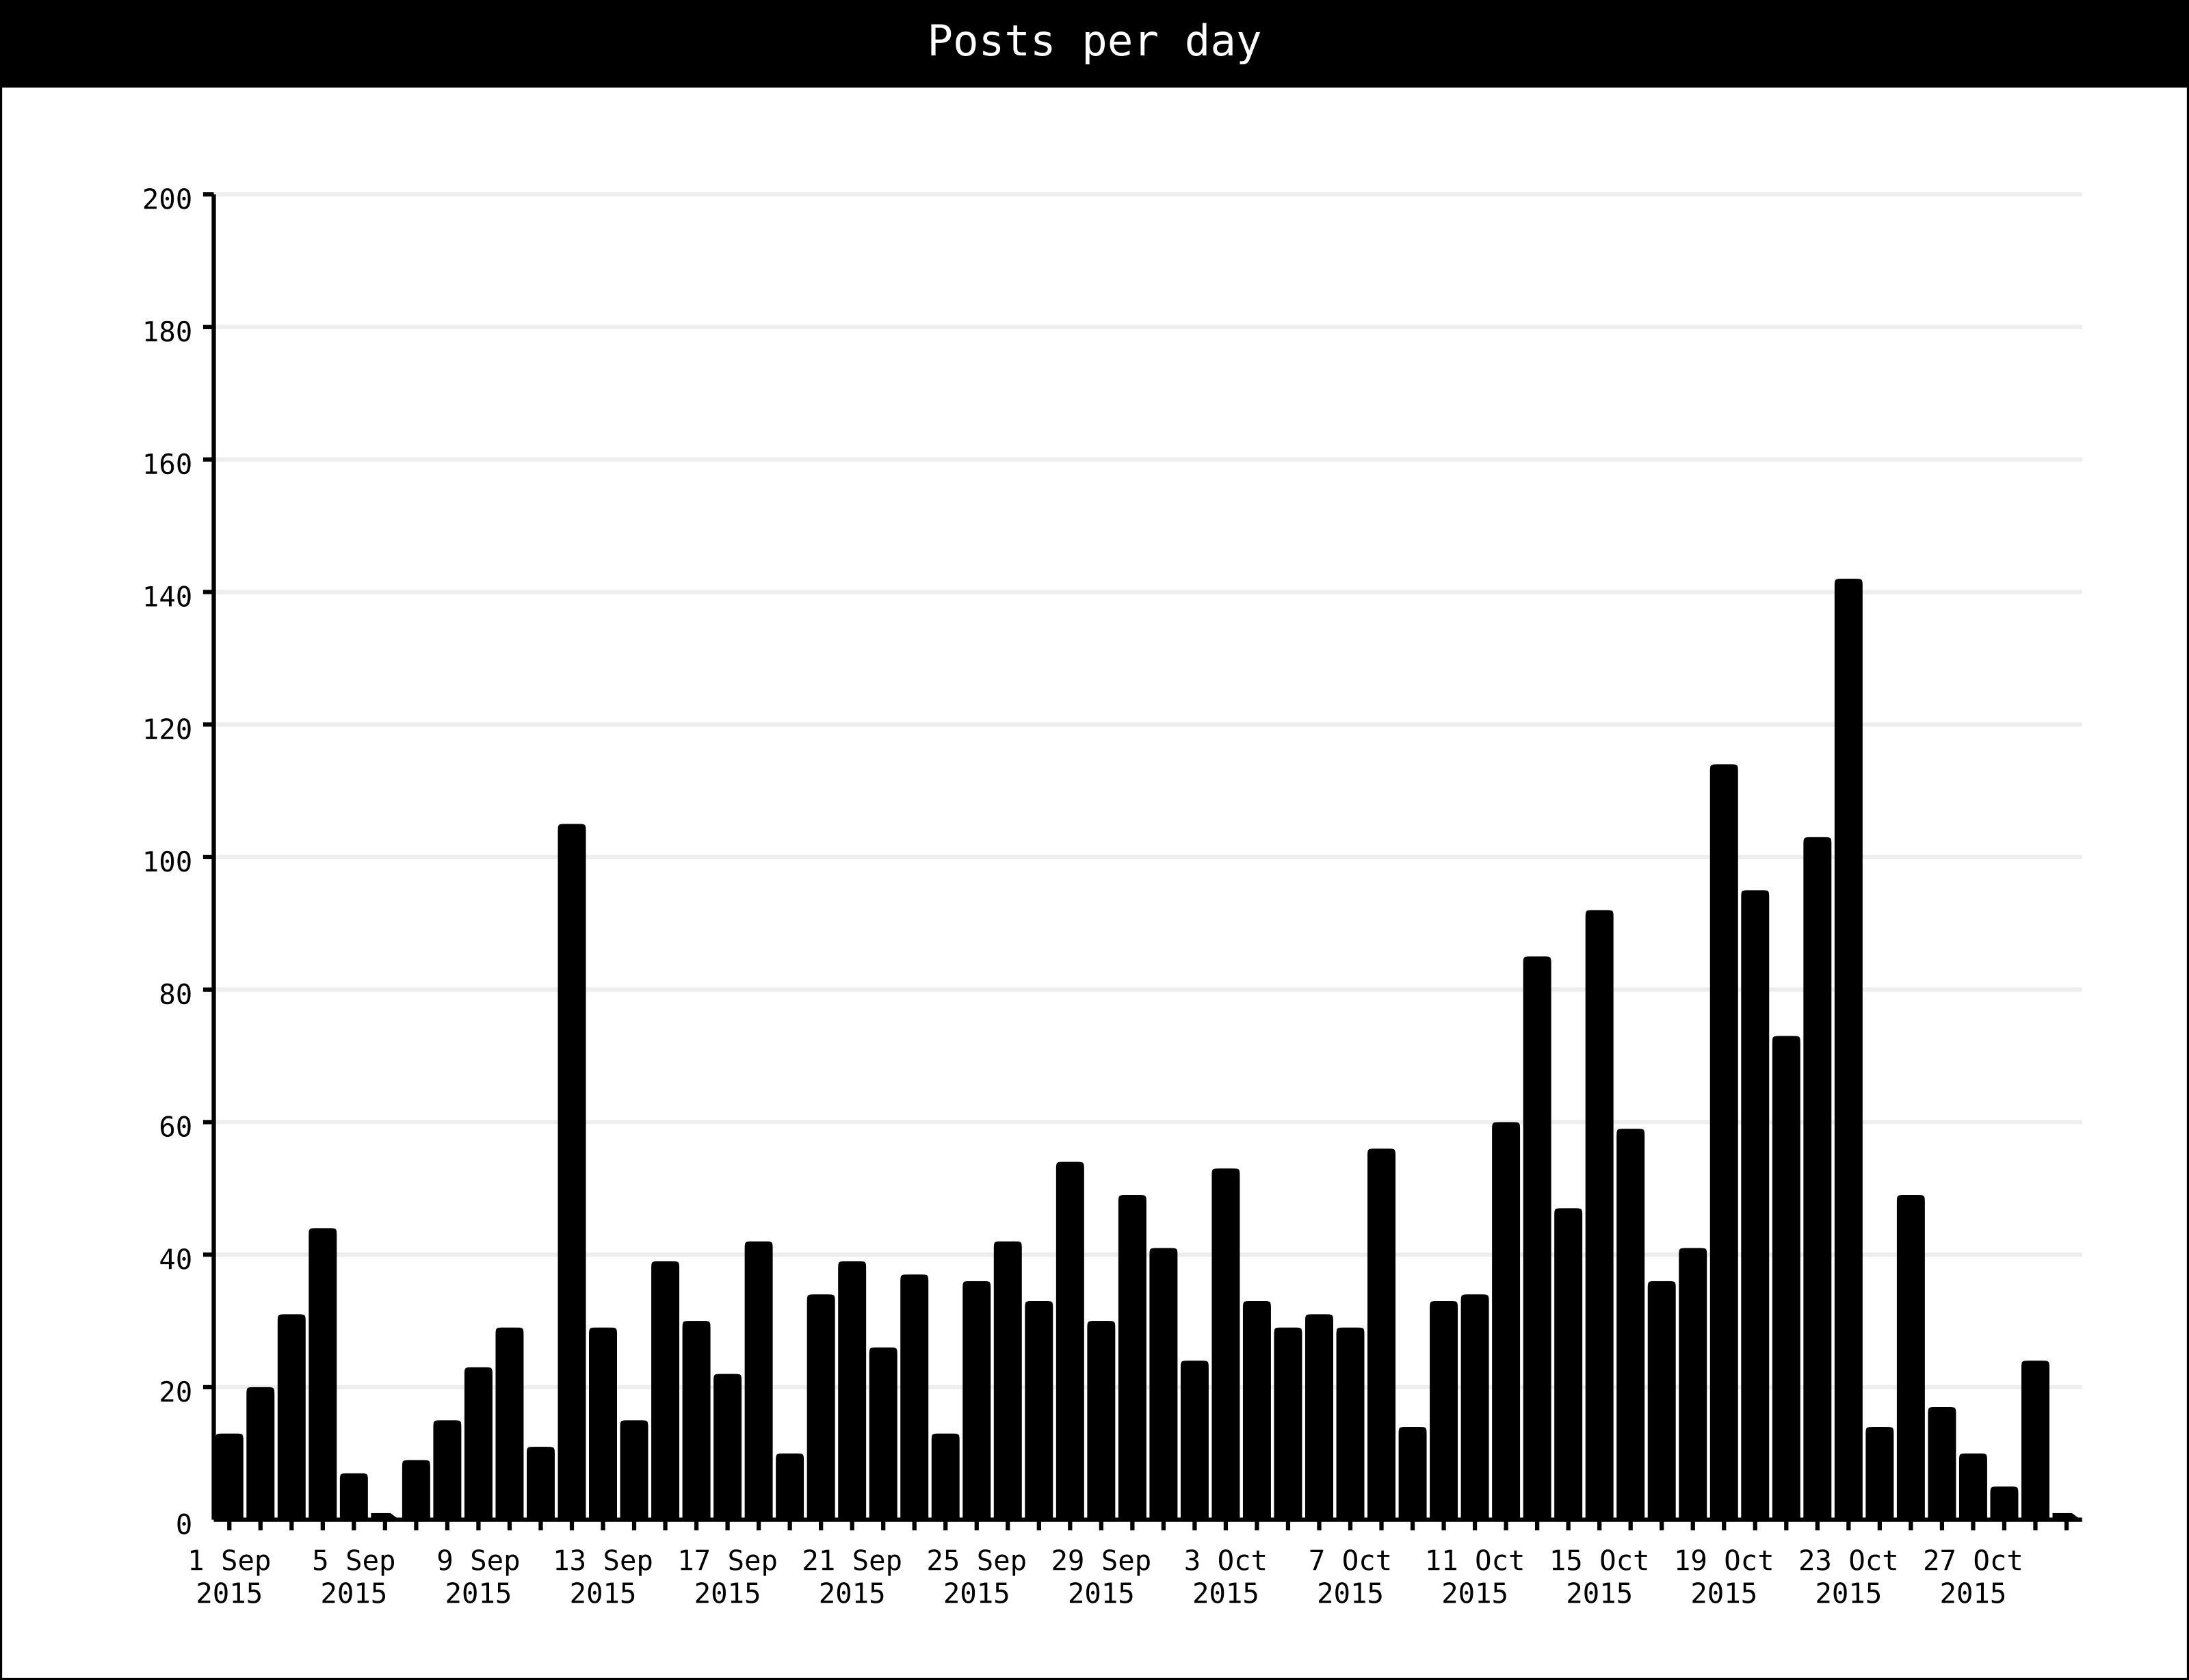
\includegraphics[width=\linewidth]{Graphics/histogram-2015.png}
\caption{Post Histogram (2015)}
\end{figure}

\pagebreak

The histogram displays the daily posts from all monitored accounts from September 1st to October 31st, 2015. Posting was modest through early September, typically below 40 per day, with a single outlier around September 12 at roughly 100 posts. From late September into October, the series rises steadily, with frequent surges in the 60-100 range. 

Activity peaks in the final campaign week (around October 19-24) at approximately 140–145 posts per day, before dropping back toward lower levels at the end of the month \citep{rybicki_2025_16933320}.

\begin{figure}[h!]
\centering
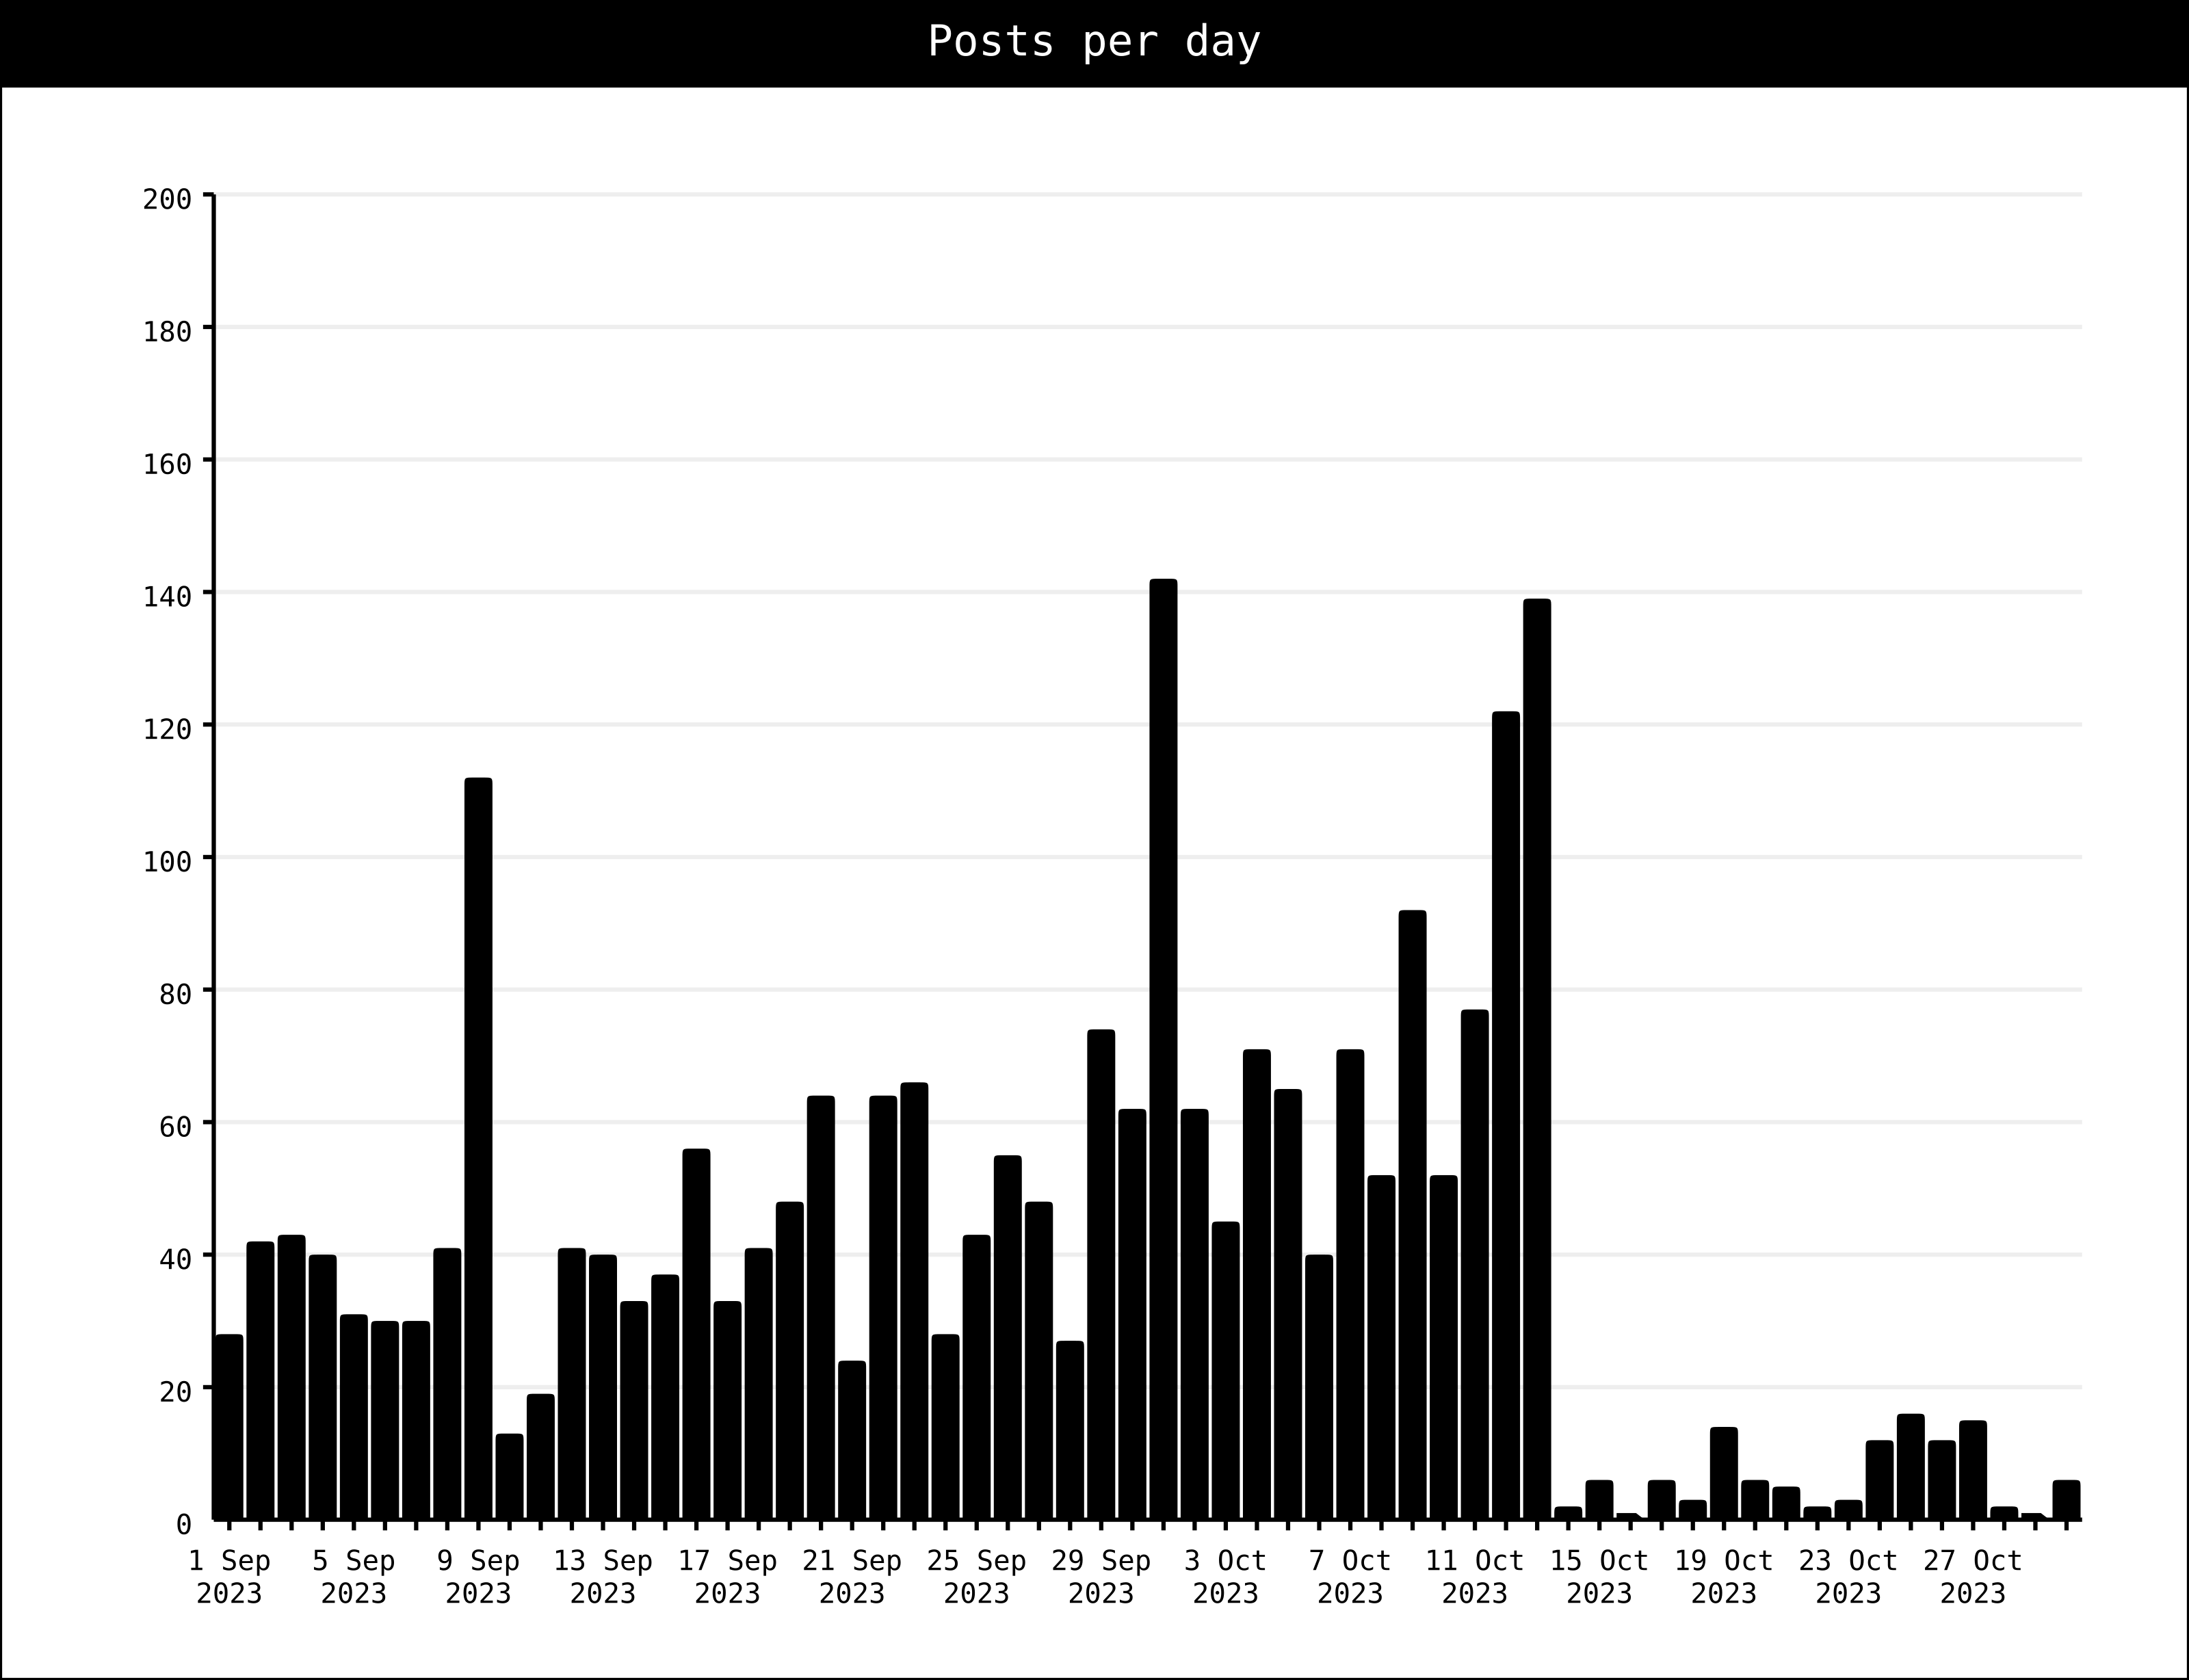
\includegraphics[width=\linewidth]{Graphics/histogram-2023.png}
\caption{Post Histogram (2023)}
\end{figure}

The histogram plots daily posts by all monitored accounts from September 1st to October 31st 2023. Activity in early September is moderate, typically between 25 and 50 posts per day, with an early spike around September 9 exceeding 110. Posting intensifies toward late September and the first half of October, with repeated surges above 70–120 and prominent peaks around late September and October 15 approaching 140 posts per day. After mid-October, the volume collapses to single digits, with only occasional small bumps below 20 through the end of the month \citep{rybicki_2025_16933320}.

\subsection{Othering}

In terms of content, a consistent feature of PiS communication since 2015 has been the construction of external and internal enemies. Russia, Germany, and the European Union emerge as recurrent foes, often linked together in a single narrative. Already during the 2015 campaign, Beata Szydło opposed the idea of a political "reset" with Russia, framing such a position as a dangerous concession by the Civic Platform (PO) government \citep{pisorgpl2015a}. In the 2023 campaign, this rhetoric was intensified and broadened, with PiS representatives repeatedly accusing PO and Donald Tusk of subordinating Poland to German and Russian interests \citep{pisorgpl2023a}. Similarly, Defence Minister Mariusz Błaszczak accused the opposition of risking national security by supposedly preparing to cede half the country to Russia \citep{pisorgpl2023b}.

Such claims often fused historical memory, sovereignty, and security concerns. For example, PiS leaders described Poland under PO–PSL rule as a "German Russian condominium," while also charging the opposition with endangering Poland's territorial integrity by allegedly considering territorial concessions to Russia \citep{pisorgpl2023c}. Furthermore, relations with neighbouring states, such as Ukraine, Lithuania, and members of the Visegrád Group, were also reframed through this lens, with PiS portraying the opposition as weakening regional alliances to the benefit of Germany and Russia \citep{pisorgpl2023d}.

Other PiS representatives further sharpened these accusations. MP Radosław Fogiel directly linked the PO government’s Russia policy to both Moscow and Berlin, emphasising German praise for Donald Tusk after the Smoleńsk disaster: 

\begin{displayquote}
    "\textit{Rząd D. Tuska prowadził wobec Rosji politykę resetu… B. Komorowski spotykał się wtedy z kanclerz Niemiec A. Merkel, która kierowała pochwały wobec D. Tuska…}" ("D. Tusk's government pursued a policy of reset towards Russia… B. Komorowski met with German Chancellor A. Merkel, who praised D. Tusk…") \citep{pisorgpl2023c}.
\end{displayquote}

\pagebreak

Prime Minister Mateusz Morawiecki complemented this narrative by embedding it in a broader populist discourse, contrasting PiS’s defence of "normality" with the alleged corruption of the opposition: 

\begin{displayquote}
    "\textit{Chcemy, aby w Polsce było normalnie - tymczasem dla Platformy normalność to obrona elit. Pieniądze szybciej uciekały z budżetu za rządów PO-PSL niż Tusk uciekł do Brukseli"} ("We want things to be normal in Poland — meanwhile, for the Platform, normality means defending the elites. Money drained from the budget faster under PO-PSL rule than Tusk fled to Brussels") \citep{pisorgpl2023d}.
\end{displayquote}

This continuity between 2015 and 2023 underscores the centrality of enemy construction in PiS's political communication. The tendency to link domestic rivals with external adversaries not only serves populist mobilisation but also anchors current conflicts in a longer historical narrative of betrayal and dependence. Across both campaigns, PiS's strategy thus reveals a striking continuity of rhetorical enemy construction, combining accusations of betrayal, foreign subordination, and the defence of corrupt elites.

PiS campaigns systematically frame Tusk and PO as political enemies, with a noticeable escalation in the number of attacks between 2015 and 2023. In 2015, party officials emphasised their confidence and dismissal of the opposition, portraying PO as non-threatening \citep{pisorgpl2015b}. In 2015, PiS politicians emphasised confidence against the opposition, with Stanisław Karczewski highlighting Beata Szydło's debate performance and declaring that the party was not afraid of PO \citep{pisorgpl2015b}. \\

\vspace{1cm}

\begin{table}[H]
    \centering
    \begin{tabular}{p{4cm}p{4cm}p{4cm}}
        \toprule
        \textbf{Phrase} & \textbf{Amount of posts 2015}  & \textbf{Amount of posts 2023} \\ \midrule
        Tusk & 1 & 220  \\
        PO & 79 & 201  \\ \bottomrule
    \end{tabular}
    \caption{Usage of "PO" and "Tusk" on Twitter/X \citep{rybicki_2025_16933320}}
    \label{tab:phrases-comp-2015-2023}
\end{table}

PiS campaigns consistently construct Donald Tusk and PO as political enemies, with a sharp increase in attack volume from 2015 to 2023. By 2023, the rhetoric had intensified. Jacek Brudziński criticised recycled opposition narratives and denounced them as "pathetic and hateful", emphasising PiS's moral and political superiority \citep{jbrudzinski2023}.

Minister of Defence Mariusz Błaszczak directly framed PiS as the guarantor of national security while blaming PO-PSL for endangering the country. He emphasised:

\begin{displayquote}
    "\textit{Zasługujemy na to, aby żyć w bezpiecznej Polsce! … To rząd PO-PSL likwidował jednostki wojskowe i narażał nas na straszne niebezpieczeństwo… Tylko wolna i suwerenna Polska jest dla nas najważniejsza!}" ("We deserve to live in a safe Poland! … It was the PO-PSL government that dismantled military units and exposed us to terrible danger… Only a free and sovereign Poland is the most important for us!") \citep{pisorgpl2023e}.
\end{displayquote}

Prime Minister Mateusz Morawiecki similarly emphasised Tusk's alleged dishonesty, portraying PiS as credible and responsible in comparison to a deceitful opposition:

\begin{displayquote}
    "\textit{Tusk ciągle kłamie… Opozycja potrafi siać chaos i zawijać dobra narodowe}" ("Tusk keeps lying… The opposition is capable of sowing chaos and plundering national assets") \citep{pisorgpl2023f}.
\end{displayquote}

Earlier statements from 2015 also portrayed Tusk and PO as untrustworthy and failing to meet the public's expectations \citep{pisorgpl2015c}. Tusk was accused of breaking tax promises and betraying public trust \citep{pisorgpl2015d}. Overall, PiS campaigns have systematically intensified the volume and frequency of attacks against Tusk and PO over the years, consistently portraying them as threats to national security, economic stability, and political credibility.

\pagebreak

\subsection{Security}

Since 2015, PiS campaigns have frequently linked Poland's security with Ukraine's, emphasising threats from Russia while framing the party as the guarantor of national safety. The frequency of security-related references shows a marked increase from 2015 to 2023, both for Russia and Ukraine. \\

\vspace{1cm}

\begin{table}[H]
    \centering
    \begin{tabular}{p{4cm}p{4cm}p{4cm}}
        \toprule
        \textbf{Phrase} & \textbf{Amount of posts 2015}  & \textbf{Amount of posts 2023} \\ \midrule
        Russia & 3 & 65  \\
        Ukraine & 1 & 83  \\ \bottomrule
    \end{tabular}
    \caption{Usage of "Russia" and "Ukraine" on Twitter/X \citep{rybicki_2025_16933320}}
    \label{tab:phrases-comp-2-2015-2023}
\end{table}

The government's proactive economic policies in response to the pandemic and the war in Ukraine are emphasised, presenting these actions as part of a broader strategy to safeguard the nation \citep{pisorgpl2023g}. Similarly, PiS MEP Beata Szydło highlighted military and civil security, stressing support for the Polish Army and uniformed services, particularly in the context of the war in Ukraine, and acknowledging the personnel protecting Poland's borders \citep{pisorgpl2023h}.

The Minister of Defence, Mariusz Błaszczak, has repeatedly criticised the previous PO-PSL government while presenting PiS as the guarantor of Poland's safety, emphasising the importance of a free and sovereign Poland and asserting that past policies exposed the country to significant risks \citep{pisorgpl2023i}.

The use of hashtags such as \textit{\#BezpiecznaPolska} (\textit{\#SafePoland}) illustrates how PiS connects these narratives of military, economic, and national security to broader social media campaigns. By linking Poland's stability with Ukraine's crisis, the party mobilises public concern while framing itself as the guarantor of safety, both digitally and rhetorically. \\

Both tables below display the most frequently used hashtags in PiS-related tweets during the 2015 and 2023 election campaigns. In both cases, \#pis was the dominant marker of party identity. In 2015, hashtags such as \#damyradę highlighted themes of perseverance, whereas in 2023, \#bezpiecznapolska and related terms emphasised multiple themes centred around security. Both lists also included election-specific hashtags \#wybory2015 and \#wybierzpis, indicating a consistent integration of direct electoral appeals. Overall, the data suggest continuity in central identifiers alongside variation in thematic framing across campaigns.

\vspace{1cm}

\begin{table}[H]
    \centering
    \begin{tabular}{p{6cm}p{3cm} }
        \toprule
        \textbf{Hashtag} & \textbf{Amount of posts} \\ \midrule
        \char"0023pis& 314  \\ 
        \char"0023damyradę& 138  \\ 
        \char"0023damyrade& 123 \\
        \char"0023konwencjapis& 100 \\
        \char"0023debata& 86 \\
        \char"0023wybory2015& 72 \\
        \char"0023po& 44 \\ 
        \char"0023 24hdlapolski& 40 \\ 
 \char"0023periscope&36\\
 \char"0023podcast&30\\ \bottomrule
    \end{tabular}
    \caption{Top Hashtags 2015}
    \label{tab:top-hashtags-2015}
\end{table}

\begin{table}[H]
    \centering
    \begin{tabular}{  p{6cm}  p{3cm} }
        \toprule
        \textbf{Hashtag} & \textbf{Amount of posts} \\ \midrule
        \char"0023pis & 344\\ 
        \char"0023bezpiecznapolska & 335\\ 
        \char"0023bezpiecznaprzyszłośćpolaków& 176\\ 
 \char"0023kaczyński&94\\
 \char"0023konkretypis&86\\
 \char"0023warszawa&85\\
 \char"0023wybierzpis&58\\
 \char"0023sejm&49\\
 \char"0023końskie&48\\
 \char"0023tylkopis&46\\ \bottomrule
    \end{tabular}
    \caption{Top Hashtags 2023}
    \label{tab:top-hashtags-2023}
\end{table}

Prime Minister and PiS President Jarosław Kaczyński emphasised the importance of engaging with Polish citizens while also memorialising figures associated with national resilience, such as Przemysław Gosiewski, who died in the Smoleńsk attack. In doing so, he framed these narratives within the broader discourse of national security, explicitly using the hashtag \textit{\#BezpiecznaPolska} to reinforce the campaign's focus on a "safe Poland" \citep{pisorgpl2023j}.

\begin{displayquote}
    "\textit{Premier, Prezes PiS Jarosław Kaczyński we Włoszczowie: „Dla nas rozmowy z Polakami są bardzo ważne. Ale będąc tutaj muszę wspomnieć o Śp. Przemysławie Gosiewskim, który zginął w zamachu smoleńskim. On pokazał, że dzięki silnej woli można dużo zrobić. \#BezpiecznaPolska}" ("Prime Minister, PiS President Jarosław Kaczyński in Włoszczowa: "For us, conversations with Poles are very important. But being here, I must mention the late Przemysław Gosiewski, who died in the Smoleńsk attack. He showed that with strong will, much can be achieved. \#BezpiecznaPolska”) \citep{pisorgpl2023j}.
\end{displayquote}

The PiS campaign not only emphasises current security and political issues but also strategically recalls historical events and national tragedies to reinforce its narrative and connect with voters emotionally. References to the Smoleńsk air disaster, the Katyń massacre, and the Solidarity movement have increased between 2015 and 2023, highlighting the party's growing use of collective memory and patriotic symbolism in its messaging. These historical touchpoints are framed as integral to Poland's identity and resilience, creating a continuity between past sacrifices and present governance.


\subsection{Commemoration}

\begin{table}[H]
    \centering
    \begin{tabular}{p{4cm}p{4cm}p{4cm}}
        \toprule
        \textbf{Phrase} & \textbf{Amount of posts 2015}  & \textbf{Amount of posts 2023} \\ \midrule
        Katyń & 0 & 1  \\
        Smoleńsk & 1 & 4  \\ 
        Solidarnosc & 16 & 23  \\ \bottomrule
    \end{tabular}
    \caption{Usage of "Katyń", "Smoleńsk" and "Solidarnosc" on Twitter/X \citep{rybicki_2025_16933320}}
    \label{tab:phrases-comp-3-2015-2023}
\end{table}

This table illustrates PiS's intensified emphasis on commemorating pivotal national moments, linking historical remembrance to contemporary political discourse.

PiS also emphasises historical memory as a key component of its political messaging, particularly by recalling traumatic events such as the Katyń massacre, the Smoleńsk air disaster, and World War II atrocities. The party frames these events as central to Polish identity and national resilience, linking past tragedies to contemporary political narratives. For example, September 17th, 1939, is highlighted as a symbolic date in Polish and European memory, referencing Katyń and other sites of Soviet crimes, illustrating the ongoing significance of historical awareness \citep{pisorgpl2023j}. Similarly, the consequences of World War II, with the current call for reparations, are being connected, emphasising that remembrance and justice remain inseparable \citep{pisorgpl2023k}. PiS President Jarosław Kaczyński also invoked the memory of Przemysław Gosiewski, who died in the Smoleńsk air disaster, framing it as a demonstration of strong will and linking it to the broader theme of national perseverance \citep{pisorgpl2023l}.

PiS also emphasises Poland's Catholic heritage in its political communication, linking faith to national identity and social cohesion. Prime Minister Mateusz Morawiecki highlighted the legacy of John Paul II, portraying him as a creator of Polish freedom and solidarity who placed Polish families at the centre of national life, framing the national community as a foundational value \citep{pisorgpl2023m}. Similarly, in 2015, a gesture by President Andrzej Duda laying flowers at the Papal Cross was framed as a tribute to John Paul II, signalling the continued symbolic importance of Catholicism in public life \citep{jbrudzinski2015}.

PiS often intertwines Catholicism and the legacy of Solidarność to reinforce a narrative of Polish independence and moral authority. Prime Minister and PiS President Jarosław Kaczyński highlighted this connection by linking the fight for national sovereignty, the work of St. John Paul II, and the Solidarność movement as foundational elements preventing Poland from becoming subordinate within the European Union:

\begin{displayquote}
    "\textit{Nie po to była walka o niepodległości, nie po to była działalność Św. Jana Pawła II i nie po to była 'Solidarność', aby stać się w UE państwem poddanym innym. My nie mamy nic przeciwko Unii Europejskiej, ale chcemy w niej znam. Nie można pozwolić na dominację jednego państwa. \#BezpiecznaPolska}" ("The fight for independence, the work of St. John Paul II, and 'Solidarity' were not for us to become a state subordinate to others in the EU. We have nothing against the European Union, but we want to be significant in it. We cannot allow one state to dominate. \#BezpiecznaPolska") \citep{pisorgpl2023n}.
\end{displayquote}

Prime Minister Mateusz Morawiecki further emphasised this relationship, expressing gratitude to Solidarność for defending the legacy of John Paul II and framing the ongoing struggle for a better Poland as a continuation of both the religious and social movement’s mission:

\begin{displayquote}
"\textit{Dziękuję Solidarności za obronę dobrego imienia i pamięci o najwybitniejszej osobie w historii świata - mowa o Janie Pawle II. Bitwa o lepszą Polskę trwa i będzie trwać. Przed ludźmi solidarności wielkie zadanie, aby obronić tego co zostało dokonane w ostatnich latach bo Polska jest najważniejsza}" ("I thank Solidarity for defending the good name and memory of the most outstanding person in the history of the world - I am speaking of John Paul II. The battle for a better Poland continues and will continue. The people of Solidarity face a great task to defend what has been achieved in recent years because Poland is the most important") \citep{pisorgpl2023o}.
\end{displayquote}

These examples illustrate how PiS frames Poland's Catholic heritage and Solidarność as mutually reinforcing pillars of national identity, sovereignty, and moral authority.

\subsection{Memory}

\begin{table}[H]
    \centering
    \begin{tabular}{p{4cm}p{4cm}}
        \toprule
        \textbf{Amount of posts 2015}  & \textbf{Amount of posts 2023} \\ \midrule
        14 & 42  \\ \bottomrule
    \end{tabular}
    \caption{Usage of "rememb*" on Twitter/X \citep{rybicki_2025_16933320}}
    \label{tab:phrases-comp-4-2015-2023}
\end{table}

Lastly, PiS's communications frequently employ memory to shape public perception of the past and present. In 2023, tweets often begin with "pamiętajcie" or "pamiętamy", emphasising the failures of opposition parties while highlighting the achievements of PiS. For example, followers were reminded to vote for PiS candidates in October 2023, framing this as a continuation of the party's positive legacy and protection of the nation \citep{pisorgpl2023p}. Other posts recalled the perceived failures of opposition governments, including unemployment, low wages, and insufficient social programs, while contrasting these with the improvements achieved under PiS rule and emphasising citizens' safety as a core value \citep{pisorgpl2023q}.

In 2015, memory-focused tweets were framed more around national pride, historical roots, and the heroism of the Polish people. Kaczyński emphasized Poland’s presence everywhere and the importance of remembering compatriots abroad: "\textit{Polska jest wszędzie, w każdej wsi i mieście. Pamiętajmy o naszych rodakach poza granicami, nie zapominajmy o korzeniach}" ("Poland is everywhere, in every village and city. Let us remember our compatriots abroad, let us not forget our roots") \citep{pisorgpl2015e}. He also highlighted moral values, urging followers to remember humility as a guiding principle for all citizens \citep{pisorgpl2015f}. In addition, he framed memory as the foundation of national identity, emphasising that the remembrance of heroes underpins Polish cultural and historical identity \citep{pisorgpl2015g}.

\pagebreak

\subsection{Outliers}

Specific patterns in the data emerge as outliers. Mentions of Smoleńsk and Solidarność were relatively infrequent, indicating that these topics may target a narrower or more specific audience than other themes. Individual accounts exhibit distinctive behaviours: President Andrzej Duda, despite having the most extensive follower base among the analysed accounts, posts the least and focuses on content that differs from other politicians. Jarosław Kaczyński appears frequently in traditional media coverage but is less prominent online, whereas Joachim Brudziński extensively uses hashtags, surpassing other accounts in both quantity and diversity. These deviations highlight how social media activity does not always mirror offline visibility or influence \citep{rybicki_2025_16933320}. 

PiS campaign narratives remained consistent between 2015 and 2023, emphasising memory, national identity, and opposition critique. However, 2023 saw a higher volume of text-heavy posts and intensified attacks on opponents, whereas 2015 relied more on images and symbolic gestures \citep{rybicki_2025_16933320}. These patterns suggest continuity in messaging strategies, with a precise amplification of themes over time, paving the way for the discussion of their impact on political mobilisation and voter engagement.



\newpage\null\thispagestyle{empty}\newpage

%CHAPTER 5
\chapter[Discussion]{Discussion}
\label{Chap:Discussion}
This chapter examines how PiS mobilises historical myths, collective trauma, and selective interpretations of national identity to consolidate political authority, delegitimise opposition, and shape public perceptions of Poland’s past and present. The discussion situates PiS within broader Central European trends of democratic backsliding, highlighting the interplay between populist rhetoric, nationalist ideology, and mnemonic governance in constructing a dominant vision of the nation.

\section{Interpretation of Results}

A central element of PiS's political discourse is the revival of historical paradigms that portray Poland as a sovereign, morally superior power resisting external domination. One prominent example is the idea of Intermarium, initially envisioned by Józef Piłsudski, which positions Poland as a pre-communist regional power countering threats from Moscow and Berlin \citep{riedel_tri-marium_2022}. PiS's election platforms actively invoke this legacy, depicting Poland as a moral and geopolitical leader in the post-Soviet space and calling for the unity of Central and Eastern European states to defend sovereignty against foreign pressures \citep{pis_program_2023}.

The 2010 Smoleńsk air crash is the most prominent example of PiS’s instrumentalisation of victimhood, transformed into a sacrosanct national trauma comparable to the Katyń massacre. This event reinforces a narrative of Soviet betrayal and eternal grief \citep{fredheim_memory_2014}. Religious and sacrificial language is used to position PiS as the rightful heir to Poland’s heroic dead and defender of national pride \citep{ksiazek_smolensk_2018}. PiS rejects the "pedagogy of shame" associated with earlier acknowledgement of Polish complicity in WWII atrocities, promoting instead a discourse of Polish innocent victimhood \citep{woycicka_mnemonic_2024}.

Catholicism is tightly woven into these historical and national narratives, framing Poland’s identity within a divine mission that legitimises assertive security policies against historic threats from Russia and Germany \citep{lazor_memory_2016}. 

\pagebreak

Public commemorations, including Katyń remembrance and national anniversaries such as the Independence March, blend pride and grief while reinforcing anxieties about sovereignty \citep{pis_program_2023}.

Katyń functions as a mnemonic hotspot, where patriotism is equated with resistance to Europeanization and perceived treason \citep{fredheim_memory_2014}. National anniversaries similarly symbolise Poland’s rebirth and struggle against foreign domination \citep{kobierecki_opportunistic_2022}.

Communism is portrayed as fundamentally alien and illegitimate, often compared to Nazism and sometimes infused with antisemitic undertones \citep{korycki_memory_2017}. This discourse constructs a narrative of victimhood, legitimising PiS’s opposition to post-communist elites. Policymakers frequently employ simplified or mythologised historical analogies to justify systemic reforms. The post-1989 democratic transition in Poland and Hungary is reinterpreted as a tale of betrayal and moral decline. This narrative is used to legitimise initiatives such as the "Fourth Republic" and a revived ethno-organic national state. Similarly, the 1989 Round Table negotiations are depicted as illegitimate by populist actors \citep{pozarlik_momentarily_2022}.

Kaczyński and PiS argue that since 1989, an "old-new elite" has monopolised political, economic, and cultural power in Poland, consisting of an alliance between post-communist and liberal post-Solidarity forces. According to the party’s 2014 program, this negative "pseudo-elite" is beholden to foreign interests, exhibits a "distaste . . . for the [Polish] state," and maintains a "suspicious attitude towards the nation" \citep{bill_counter-elite_2022}. Kaczyński contends that liberal civil society, media, and cultural elites share this outlook, often rejecting the very concept of the nation. These groups, he claims, submissively emulate Western trends in ways that betray authentic Polish interests and values. The "pseudo-elite" must therefore be replaced by a "counter-elite," a set of PiS-aligned groups dedicated to promoting national interests. In this sense, PiS’s populism is a form of "counter-elite" populism; it is not inherently anti-elite. Instead, it defines a fundamental conflict between a false elite and the people, who are represented by the true (counter-)elite \citep{bill_counter-elite_2022}.

This framing is echoed in recent statements by PiS leaders. For example, Minister Czarnek asserted that if Tusk had been in power during Russia’s attack on Ukraine, genocidal forces would have reached Poland, and eastern Poland would have continued to lack investment and infrastructure \citep{pisorgpl2023p}. Similarly, Kaczyński warned that a return to Tusk’s leadership would revive past chaos, plundering, and subordination to Brussels and Germany, emphasising that PiS governs independently as a free and sovereign nation \citep{pisorgpl2023q}. Kaczyński further claimed that Tusk’s party is "external," effectively German, seeks to undermine democracy, employs thuggish methods, and relies solely on lies \citep{pisorgpl2023r}.

The legacy of Solidarność, while not always explicitly invoked, remains central in legitimising Poland’s post-1989 identity as an anti-communist bastion \citep{piotrowski_between_2010}. PiS construes Solidarność as a fixed symbol of conservative nationalism, truncating its original, inclusive social movement origins \citep{piotrowski_between_2010}. Earlier governments had presented Solidarność in a more pluralistic manner, emphasising inclusivity and pro-European values \citep{woycicka_mnemonic_2024}. This selective narrative sidelines progressive and minority voices, consolidating conservative interpretations of history and limiting space for dissent \citep{assmann_transnational_2014}. PiS’s politics of memory deliberately reinforce a singular vision of national history based on heroism, martyrdom, and victimhood, excluding alternative perspectives \citep{mazzini_three-dimensional_2018}. Commemoration is repoliticized, portraying Poland as a perennial victim of communism and moral decay under post-1989 democratic elites, whom the party frames as traitors \citep{lazor_memory_2016}. PiS’s mnemonic warfare strategy is not merely tactical; it is integral to its broader ideological project of building a "Fourth Republic," framing memory as an existential imperative and moral obligation necessary for national renewal.

Their mythologised narratives also serve contemporary political purposes, particularly in delegitimising opposition. The Smoleńsk discourse frames Civic Platform and Donald Tusk as betrayers of Polish sovereignty \citep{ksiazek_smolensk_2018}. By selectively highlighting Solidarność’s conservative aspects and marginalising liberal and minority perspectives, PiS consolidates its nationalist ideology while minimising opportunities for critical reflection or dissent \citep{piotrowski_between_2010}. Solidarność is made central to conservative nationalism through the exclusion of liberal and minority voices \citep{lazor_memory_2016}.

Their mythologised narratives also serve contemporary political purposes, particularly in delegitimising opposition. The Smoleńsk discourse frames Civic Platform and Donald Tusk as betrayers of Polish sovereignty \citep{ksiazek_smolensk_2018}. By selectively highlighting Solidarność’s conservative aspects and marginalising liberal and minority perspectives, PiS consolidates its nationalist ideology while minimising opportunities for critical reflection or dissent \citep{piotrowski_between_2010}. Solidarność is made central to conservative nationalism through the exclusion of liberal and minority voices \citep{lazor_memory_2016}.

From 2015 to 2023, PiS increasingly positioned itself as reclaiming Poland’s national sovereignty and dignity from foreign domination, combating EU federalism and political homogenisation, and advancing military and diplomatic strength to protect regional stability \citep{pis_program_2023}. It framed the EU as a neo-imperial hegemon and cast itself as the leader of a coalition resisting ideological domination from Brussels \citep{riedel_tri-marium_2022}. 

\pagebreak

Political opponents were othered as foreign elites hostile to "true Poles," legitimising their exclusion and the concentration of power \citep{siedlicka_pis_2015}. These discourses supported the consolidation of political authority \citep{wronski_pis_2015}.

\section{Relating to Literature}

Since 2015, PiS has evolved from its earlier "memory warrior" phase (2005–2007) into a more radical form. The party acts as a memory excluder and implements systematic mnemonic politics across domestic and foreign policy spheres \citep{mazzini_three-dimensional_2018}. Guided by a "politics of certainty," PiS frames itself as the sole guardian of authentic national identity. It also positions itself as the revealer of hidden truths about a betrayed political transition \citep{dujisin_reassessing_2024}. Following 2010, and especially after the Smoleńsk tragedy, PiS militarised memory through the takeover of public institutions. This memory regime envisions Poland as a heroic nation under siege. It legitimises illiberal governance and disenfranchises opposition \citep{woycicka_mnemonic_2024}.

Poland’s post-EU accession period initially witnessed a permissive, inclusive memory culture promoted by civil society and NGOs \citep{stanczyk_commemorating_2014}. PiS’s return to government marked a shift toward a closed, exclusionary model of memory governance, creating a deep divide between liberal and illiberal historical narratives \citep{stanczyk_commemorating_2014}. The party constructs an existential political myth of struggle between "true Poles" and corrupt post-communist elites. This myth instrumentalises collective memory for political purposes \citep{korycki_memory_2017}.

Institutional reforms support memory work beyond nationalist narratives, recuperating concepts such as "Piast Poland" and the "recovered territories" to cement German guilt and Polish victimhood \citep{langenbacher_twenty-first_2008}. Similarly, the party frames its refusal to sign international climate treaties as a defence of Polish sovereignty against global Others, reinforcing nationalist identity through climate change denial \citep{ulanowski_pis_2015}.

The EU is perceived as remote and abstract, failing to foster a habitual and emotional attachment \citep{jamieson_theorising_2002}. Populist and nationalist movements, such as PiS, exploit this gap to reject supranational identities \citep{jamieson_theorising_2002}.

PIS´s strategy exemplifies the ideocratic turn in Central Europe. Democratic systems are transformed into illiberal, majoritarian regimes through a combination of populist rhetoric, nationalist memory politics, and ideological reinterpretation of history \citep{rupnik_crisis_2018}. The outcome is a mnemonic order in which dissent is treated as treason. Memory becomes ideology. The national "self" is continuously reinforced through the exclusion and vilification of the "other" \citep{mazzini_three-dimensional_2018}. These myths consolidate a Polish martyrological identity \citep{meijen_populist_2024}, through which Poland is consistently portrayed as the noble victim of Nazi and Soviet aggression \citep{gliszczynska_grabias_memory_2014}.

PiS populism is strongly tinged with nationalism \citep{brubaker_populism_2020}. Traditional Polish scholarship often defines nationalism narrowly in terms of pre-war National Democracy \citep{cordell_transformation_2015}. This thesis adopts a broader conception: loyalty to the nation takes precedence over other collective loyalties. Thus, the nation is the sole source of legitimate political authority \citep{jaskulowski_populist_2023}.


\section{Practical Impact}

From 2015 to 2023, the Law and Justice Party (PiS) consistently integrated its electoral programs into a nationalist-leaning ideology through the use of memory politics. Using populist rhetoric and anti-elitist messaging, PiS mobilises support by portraying ordinary Poles as reclaiming a history allegedly distorted by cosmopolitan elites, while minimising the experiences and agency of lower social classes \citep{jaskulowski_populist_2023}.

PiS presents history as a narrative of national heroes defending an ethnically homogeneous nation that is always a victim rather than an aggressor, using this memory politics as a tool of social pedagogy. Its nationalist ideology paradoxically frames national identity as deeply rooted yet insufficiently recognised by the populace, necessitating promotion by a self-proclaimed “authentic national elite” through education, media, and culture \citep{jaskulowski_populist_2023}. In countries such as Russia, Hungary, and Poland, conspiratorial narratives suggested that Western financial institutions and political elites, termed the “wrong elite”,  orchestrated the collapse of communism to plunder national resources and impose cultural dominance \citep{bergmann_strategic_2025}.

Elections are framed not as instruments of representation but as subordinate to the authority of elites interpreting the nation’s authentic identity; those who resist this vision face exclusion and pressure. Overall, PiS’s memory politics exemplifies its radical nationalist character, using populist strategies to foster national cohesion, cultural consolidation, and moral renewal \citep{jaskulowski_populist_2023}.


\newpage\null\thispagestyle{empty}\newpage

%CONCLUSION CHAPTER
\chapter[Conclusion]{Conclusion}
\label{Chap:Conclusion}

This study demonstrates that the collective memory politics of Law and Justice (PiS) during its 2015 to 2023 election campaigns are marked by both continuity and change. Certain mnemonic tropes, othering, victimhood, nationalism, Catholicism, and commemoration, remain central and stable over time, forming the ideological backbone of PiS’s project of national identity construction \citep{zuk_anti-semitic_2023}. These elements provide a coherent narrative framework that consistently divides society into "true Poles" and ideological or foreign "others" \citep{kapralski_jews_2017}. Such continuity underscores the durability of populist identity politics that are deeply anchored in emotionally charged historical narratives \citep{couperus_memory_2023}.

The resulting mythologised narratives consolidate a Polish martyrological identity, portraying Poland as a noble victim of Nazi and Soviet aggression while often overlooking historical complexities and uncomfortable truths regarding Polish complicity \citep{meijen_populist_2024}. The myth of a "heroic and noble Poland", devoid of "black spots" in its history, simplifies the past to protect nationalist innocence and suppress pluralistic or critical interpretations \citep{zuk_anti-semitic_2023}. At the heart of this mnemonic conflict lies a contestation over Poland’s recent past, where competing narratives of heroism, victimhood, and marginalisation expose deep social fractures \citep{piotrowski_between_2010}. 

Thus, PiS’s narrative establishes a persistent "us versus them" cleavage. The party positions itself as the sole defender of Polish sovereignty, identity, and traditional values, setting itself against other opposition parties and supranational entities. By invoking historical memory and cultural continuity, PiS mobilises support and portrays Poland as a resilient nation resisting both external domination and internal decay \citep{woycicka_mnemonic_2024}. Across electoral cycles, memory serves both as a tool for national unity and as a means of ideological legitimation. The 2023 cycle reflects more pervasive and organised memory politics as a method of ideological control \citep{rybicki_2025_16933320}, a concern echoed by liberal media and opposition actors \citep{woycicka_mnemonic_2024}.

Nevertheless, within this continuity lies a significant change in emphasis, intensity, and medium. While the Smoleńsk tragedy operated as a constitutive myth in the 2015 campaign, ritualised in commemorations and heavily featured in political discourse, by 2023 its explicit centrality had diminished \citep{rybicki_2025_16933320}. Its symbolic weight, however, persisted as a background reference point, embedded within broader narratives of martyrdom and Polish victimhood \citep{woycicka_mnemonic_2024}. More decisive is the transformation in how PiS deploys memory politics: the digital sphere, and especially social media, has become a primary stage for advancing mnemonic narratives \citep{jamieson_theorising_2002}. On these platforms, repetition, speed, and emotional immediacy enable PiS to normalise exclusionary rhetoric and disseminate nationalistic frames with a far greater reach. The tone has also grown more aggressive, leveraging the affordances of digital media to intensify polarisation and diminish the legitimacy of dissent \citep{meijen_populist_2024}.

Politically, these memory practices serve a dual purpose. First, they reinforce PiS’s claim to domestic legitimacy, presenting the party as the sole custodian of Poland’s historical truth and moral identity \citep{korycki_memory_2017}. Second, they function to delegitimize opponents by collapsing a wide spectrum of adversaries,  Civic Platform (PO), Russia, Germany, and the EU, into a single symbolic enemy \citep{mazzini_three-dimensional_2018}. This strategy of amalgamation simplifies political conflicts into a stark moral binary, sustaining a siege mentality and fortifying in-group cohesion \citep{bernhard_notitle_2014}. By fusing disparate threats into one melting pot of hostile "others", PiS effectively weaponizes memory politics as a populist tool of mobilization and governance \citep{woycicka_mnemonic_2024}.

The findings also highlight broader implications for the study of populism and collective memory. PiS’s ability to institutionalize mnemonic politics, through commemorations, legislative measures, and control of public media, demonstrates how memory regimes can be transformed into enduring instruments of political legitimacy \citep{zuk_anti-semitic_2023}. In doing so, the party not only shapes historical consciousness but also actively reconfigures national identity in ways that exclude pluralistic interpretations and demonize perceived outsiders \citep{mazzini_three-dimensional_2018}.

Future research should build on the Large Language Model dataset generated for this thesis, which provides a promising methodological tool for tracing the circulation and transformation of mnemonic narratives across digital platforms. One particularly intriguing avenue is to explore how PiS’s strategy of collapsing multiple adversaries into one symbolic "other" operates in different contexts and how this shapes both domestic politics and Poland’s international positioning \citep{rybicki_2025_16933320}. This would allow scholars to better understand not only the tactical use of memory politics but also the deeper structural role of digital media in enabling populist parties to entrench exclusive and antagonistic visions of national identity. Strengthening historical literacy remains an urgent task, as greater awareness of the complexity of the past can empower both policymakers and citizens to resist oversimplified, exclusionary narratives and foster a more pluralistic, democratic debate about history and identity \citep{mumford_parallels_2015}.
 

\newpage\null\thispagestyle{empty}\newpage
\newpage\null\thispagestyle{empty}\newpage

\printbibliography

\appendix

% ***************************************************
% Appendix
% ***************************************************
\makeatletter
% Patch list of figures
\renewcommand{\listoffigures}{%
  \section{\listfigurename}%
  \@mkboth{\listfigurename}{\listfigurename}%
  \@starttoc{lof}%
}

% Patch list of tables
\renewcommand{\listoftables}{%
  \section{\listtablename}%
  \@mkboth{\listtablename}{\listtablename}%
  \@starttoc{lot}%
}
\makeatother

\appendix

\appendix
\AppChapter{}

\renewcommand{\listfigurename}{Table of Figures}
\listoffigures

\clearpage

\renewcommand{\listtablename}{Table of Tables}
\listoftables

\AppChapter{}

\section{System Setup and Configuration}

\subsection{LM Studio Installation with CUDA Acceleration}

LM Studio was installed on a Windows workstation with the following hardware:

\begin{itemize}
    \item Intel Core i7-9700K processor
    \item 32\,GB DDR4 RAM
    \item NVIDIA GeForce RTX~2080 GPU (8\,GB VRAM)
\end{itemize}

The installation process was as follows:

\begin{enumerate}
    \item \textbf{NVIDIA driver and CUDA installation} \\
    The NVIDIA driver was updated to the latest version, and CUDA~12 was installed using the official Windows installer packages. 
    Installation was verified with \texttt{nvidia-smi}, which is included with the driver and can be run from the command line.

    \item \textbf{LM Studio installation} \\
    LM Studio was downloaded from the official distribution and installed using the Windows installer.

    \item \textbf{Model download and execution} \\
    The desired model was obtained directly through the LM Studio interface. 
    GPU inference was automatically enabled and confirmed operational with the RTX~2080.

    \item \textbf{API server configuration} \\
    Within LM Studio, the API server was enabled to allow external applications to send inference requests.
\end{enumerate}

\subsection{4CAT Deployment on Windows with Docker Desktop}

4CAT was deployed on a laptop running Windows 11 using Docker Desktop. The procedure was as follows:

\begin{enumerate}
    \item \textbf{Docker Desktop installation} \\
    Docker Desktop was installed, providing both the Docker Engine and Docker Compose.

    \item \textbf{Repository setup} \\
    The 4CAT repository was downloaded from GitHub via \texttt{git} using Git Bash:
    \begin{verbatim}
    git clone https://github.com/digitalmethodsinitiative/4cat.git
    \end{verbatim} 

    \item \textbf{Configuration} \\
    A \texttt{.env} file was created from the provided template and adjusted minimally to configure authentication and database storage. 
    The service was configured to run on port~80.

    \item \textbf{Service orchestration} \\
    The repository directory was opened in PowerShell, and the services were started with:
    \begin{verbatim}
    docker compose up -d
    \end{verbatim} 

    \item \textbf{Verification} \\
    The application was made available locally at \url{http://localhost/} 

    \item \textbf{Connecting to LM Studio} \\
    To enable integration with LM Studio, the API server had to be enabled first within LM Studio. 
    The API base path (consisting of the workstation IP address followed by \texttt{/v1}) was then provided in the 4CAT interface under the options for the "LLM prompting" task. 
    This allowed 4CAT to route inference requests directly to the LM Studio backend.
\end{enumerate}


\AppChapter{}

\section{Non-exclusive licence to reproduce the thesis and make the thesis public}

I, Viktoria Rybicki,

\begin{enumerate}[nosep]
\item grant the University of Tartu a free permit (non-exclusive licence) to reproduce, for the purpose of preservation, including for adding to the digital archives of the University of Tartu until the expiry of the term of copyright, my thesis \vspace{0.3cm}

\textbf{PiS as Mnemonic Warriors: A Comporative Analysis of Changes and Continuity of Memory Narratives in the Election Campaigns 2015 and 2023} \\[0.3cm]
Supervised by: Louis Wierenga, PhD candidate, University of Tartu \&
Dr. Grzegorz Pożarlik, Jagellonian University \vspace{0.3cm}

\item grant the University of Tartu the permit to make the thesis specified in point 1 available to the public via the web environment of the University of Tartu, including via the digital archives, under the Creative Commons licence \textbf{CC BY NC ND 4.0}, which allows, by giving appropriate credit to the author, to reproduce, distribute the work and communicate it to the public, and prohibits the creation of derivative works and any commercial use of the work from 25/08/2025 until the expiry of the term of copyright; \vspace{0.3cm}

\item am aware that the author retains the rights specified in points 1 and 2; \vspace{0.3cm}

\item confirm that granting the non-exclusive licence does not infringe other persons’ intellectual property rights or rights arising from the personal data protection legislation. \vspace{0.3cm}

\end{enumerate}

\vfill

Viktoria Rybicki, 25/08/2025 \\

\end{document}